% ------------------------------------------------------------------------
% ------------------------------------------------------------------------
% ICMC: Modelo de Trabalho Acadêmico (tese de doutorado, dissertação de
% mestrado e trabalhos monográficos em geral) em conformidade com 
% ABNT NBR 14724:2011: Informação e documentação - Trabalhos acadêmicos -
% Apresentação
% ------------------------------------------------------------------------
% ------------------------------------------------------------------------

% Opções: 
%   Qualificação          = qualificacao 
%   Curso                 = doutorado/mestrado/tcc
%   Situação do trabalho  = pre-defesa/pos-defesa (exceto para qualificação)
%   Versão para impressão = impressao
\documentclass[mestrado, pre-defesa]{packages/icmc}
% ---------------------------------------------------------------------------
% Pacotes Opcionais
% ---------------------------------------------------------------------------
\usepackage{rotating}                       % Usado para rotacionar o texto
\usepackage[all,knot,arc,import,poly]{xy}   % Pacote para desenhos gráficos
\usepackage{lipsum}                         % Usado para adicionar texto temporario
\usepackage{pgf-pie}                        % Usado para adicionar gráficos de pizza
\usepackage[section]{placeins}              % Usado para manter imagens e tabelas dentro da seção
%\usepackage[subsection]{placeins}          % Usado para manter imagens e tabelas dentro da subseção
% Este pacote pode conflitar com outros pacotes gráficos como o ``pictex''
% Então é necessário usar apenas um dos pacotes conflitantes
\newcommand{\VerbL}{0.52\textwidth}
\newcommand{\LatL}{0.42\textwidth}
% ---------------------------------------------------------------------------


% ---
% Informações de dados para CAPA e FOLHA DE ROSTO
% ---
% Tanto na capa quanto nas folhas de rosto apenas a primeira letra da primeira palavra (ou nomes próprios) devem estar em letra maiúscula, todas as demais devem ser em letra minúscula.
\tituloPT{Câmaras de Eco nas Mídias Sociais: Análise de Rede do Aplicativo Colab.re}
\tituloEN{Echo Chambers in Social Media: Network Analysis of Colab.re app}
\autor[Sousa, J. G. R.]{João Guilherme Ribeiro de Sousa}
\genero{M} % Gênero do autor (M = Masculino / F = Feminino)
\orientador[Orientador]{Prof. Dr.}{Erico Souza Teixeira}
\coorientador{Prof. Dr.}{Onício Leal Neto}
\curso{CCMC}
\data{15}{06}{2023} % Data do depósito
\idioma{PT} % Idioma principal do documento (PT = português / EN = inglês)
% ---


% ---
% RESUMOS
% ---

% Resumo em PORTUGUÊS
% conter no máximo 500 palavras
% conter no mínimo 1 e no máximo 5 palavras-chave
\textoresumo[brazil]{
    Este artigo explora a natureza das câmaras de eco no aplicativo Colab.re, investigando a estrutura e a dinâmica das redes partidárias e o impacto da polarização partidária na deliberação pública. Com base em métodos da epidemiologia digital e da análise de redes, o estudo desenvolve um quadro para detectar e mitigar os efeitos das câmaras de eco no aplicativo Colab.re. Os resultados revelam a existência de grupos altamente polarizados, com interação limitada entre facções opostas, e destacam o papel da curadoria algorítmica e do comportamento do usuário na formação do ecossistema de informações. O estudo também propõe um conjunto de intervenções, incluindo sugestões de rede e moderação de conteúdo, para promover uma maior diversidade de pontos de vista e aprimorar a qualidade da deliberação pública no aplicativo Colab.re. O artigo conclui discutindo as implicações mais amplas do estudo para a governança participativa e os desafios de promover o engajamento democrático em um ambiente midiático polarizado.
    }{Análise de Redes Sociais; Câmaras de Eco; Teoria dos Grafos}


% resumo em INGLÊS
% conter no máximo 500 palavras
% conter no mínimo 1 e no máximo 5 palavras-chave
\textoresumo[english]{
    This paper explores the nature of echo chambers in the Colab.re app, investigating the structure and dynamics of partisan networks and the impact of partisan polarization on public deliberation. Drawing on methods from digital epidemiology and network analysis, the study develops a framework for detecting and mitigating the effects of echo chambers in the Colab.re app. The findings reveal highly polarized clusters with limited interaction between opposing factions and shed light on the role of algorithmic curation and user behavior in shaping the information ecosystem. The study also proposes a set of interventions, including network nudges and content moderation, to foster a greater diversity of viewpoints and enhance the quality of public deliberation in the Colab.re app. The paper concludes by discussing the broader implications of the study for participatory governance and the challenges of promoting democratic engagement in a polarized media environment.
    }{Social Network Analysis; Echo Chambers; Graph Theory}


% ----------------------------------------------------------
% ELEMENTOS PRÉ-TEXTUAIS
% ----------------------------------------------------------

% Inserir a ficha catalográfica
%\incluifichacatalografica{tex/pre-textual/ficha-catalografica.pdf}

% DEDICATÓRIA / AGRADECIMENTO / EPÍGRAFE
\textodedicatoria*{tex/pre-textual/dedicatoria}
\textoagradecimentos*{tex/pre-textual/agradecimentos}
\textoepigrafe*{tex/pre-textual/epigrafe}

% Inclui a lista de figuras
\incluilistadefiguras

% Inclui a lista de tabelas
\incluilistadetabelas

% Inclui a lista de quadros
%\incluilistadequadros

% Inclui a lista de algoritmos
%\incluilistadealgoritmos

% Inclui a lista de códigos
\incluilistadecodigos

% Inclui a lista de siglas e abreviaturas
\incluilistadesiglas

% Inclui a lista de símbolos
\incluilistadesimbolos

% ----
% Início do documento
% ----
\begin{document}
% ----------------------------------------------------------
% ELEMENTOS TEXTUAIS
% ----------------------------------------------------------
\textual

\chapter{Introdução}
\label{chapter:01_introducao}
A interação entre o ser humano e sua realidade tecnológica tem sido um tema de reflexão constante. Como argumentado por Martin Heidegger em "O Ser e o Tempo", a qualidade de nossa experiência está intrinsecamente ligada à forma como nos relacionamos com o ambiente, incluindo o uso de tecnologia. Suas observações fenomenológicas revelam que uma interação perfeita com uma ferramenta pode alterar nossa percepção existente, levando-nos a gostar e apreciar algo por reconhecê-lo e dominar seu uso \cite{2012_Silva_DISSERTATION}.

Essa compreensão de Heidegger sobre a interação com as ferramentas tecnológicas encontra ecos em pesquisas recentes em neurofisiologia, psicologia e neuropsicologia, que mostram que o uso de ferramentas para alcançar objetivos distantes desencadeia mudanças nas redes neurais responsáveis por manter um mapa atualizado da forma e postura do corpo, conhecido como "esquema corporal" na neurologia clássica. 

No estudo "Tools for the Body" \cite{2004_Maravita}, que aprofunda a análise da relação entre as ferramentas e o corpo humano, é explorado como as ferramentas tecnológicas podem se tornar extensões do corpo, ampliando nossas habilidades e transformando nossa experiência cotidiana. O autor destaca a importância da interação eficiente com as ferramentas digitais para o sucesso na manipulação do ambiente tecnológico, ressaltando que essa interação pode resultar em uma mudança significativa em nossa percepção e apreciação de marcas e serviços.

Ao considerarmos uma intersecção entre as ideias de Heidegger e o estudo contemporâneo dessas ferramentas tecnológicas, percebemos a relevância do conceito de Zuhandenheit, que descreve a tecnificação das mãos, ou seja, como as ferramentas se integram em nossas atividades cotidianas de forma fluida e transparente. No entanto, essa tecnificação excessiva das mãos em tempos contemporâneos pode levar à inautenticidade, à perda de uma conexão genuína com nosso ser e ao surgimento de um sentimento de ansiedade.

Nesse contexto, a hauntologia de Jacques Derrida oferece uma perspectiva interessante. A hauntologia descreve o estado de assombração causado pela sensação de que o presente não corresponde às promessas do passado. Em relação à tecnologia, a hauntologia nos lembra de como as interações digitais, embora aparentemente numerosas e eficientes, podem falhar em suprir as necessidades humanas básicas de conexão e pertencimento. Assim como Heidegger nos alertou sobre a tecnificação excessiva, Derrida nos convida a refletir sobre como as interações tecnológicas fantasmagóricas nos informam sobre a falta de autenticidade em nosso envolvimento com o mundo digital.

Embora essas plataformas tenham o potencial de aumentar o engajamento político e fomentar o diálogo, também são palco de um fenômeno preocupante: as câmaras de eco. Nas câmaras de eco, os usuários são expostos apenas a informações que confirmam suas crenças e tendências pré-existentes, contribuindo para a polarização das opiniões. Essa fragmentação das fontes de informação, descrita por Heidegger como uma forma de inautenticidade, e o fenômeno das bolhas de filtro, estudado por pesquisadores contemporâneos, compartilham características semelhantes e agravam o problema.

A inautenticidade, conceito central na filosofia de Heidegger, pode ser entendida como a falta de uma relação autêntica com o mundo e consigo mesmo. No contexto das plataformas de mídia social, a inautenticidade pode se manifestar quando os usuários adotam opiniões populares ou polêmicas para se encaixar em determinados grupos ou para ganhar aprovação e validação social. Essa busca por aceitação pode levar à polarização, à medida que as pessoas se alinham cada vez mais com visões extremas para se distinguir e ganhar reconhecimento dentro de suas comunidades online.

Essa tendência à inautenticidade é agravada pelos algoritmos das plataformas de mídia social, que personalizam o conteúdo exibido aos usuários com base em seu comportamento passado. Esses algoritmos, em busca de maximizar o engajamento e o tempo gasto nas plataformas, analisam o histórico de navegação, curtidas, compartilhamentos e interações do usuário para determinar quais conteúdos são mais propensos a serem do seu interesse. Como resultado, os usuários são apresentados principalmente a informações que se alinham com suas preferências e visões de mundo, enquanto conteúdos divergentes ou contraditórios são filtrados ou recebem menos destaque.

O processo de filtragem cria uma "bolha" em torno de cada usuário, onde seu ambiente de informações se torna cada vez mais estreito e alinhado com suas perspectivas existentes. Pesquisas recentes informam a noção que a formação de bolhas de filtro é um processo complexo que envolve vários fatores. De acordo com o estudo de \citeonline{2011_Pariser_BOOK}, as bolhas de filtro são criadas por algoritmos de personalização que selecionam o conteúdo com base no comportamento passado do usuário, suas conexões sociais e suas preferências expressas. Isso resulta em um ambiente de informação que é altamente personalizado e alinhado com as visões existentes do usuário.

No entanto, a formação de bolhas de filtro não é apenas uma consequência direta da personalização, mas também é influenciada pela interação do usuário com a plataforma. O estudo de \citeonline{2018_Aslay} destaca que a exposição do usuário a diferentes pontos de vista é limitada não apenas pelos algoritmos de personalização, mas também pela probabilidade do usuário compartilhar ou interagir com um conteúdo específico. Isso significa que as bolhas de filtro são reforçadas tanto pelos algoritmos de personalização quanto pelo comportamento do usuário.

Além disso, um estudo recente de \citeonline{2022_Boeker} sobre o TikTok oferece uma visão mais detalhada sobre como as bolhas de filtro são criadas nesta plataforma específica. Eles descobriram que o algoritmo de recomendação do TikTok leva em consideração várias características do usuário, como idioma, localização, ações de curtir e seguir, e taxa de visualização de vídeo. Além disso, o algoritmo também considera as tags descritivas atribuídas aos vídeos com base em análises de visão computacional, hashtags mencionadas, descrição do post, som e textos incorporados. Isso sugere que a formação de bolhas de filtro é um processo multifatorial que envolve tanto a personalização algorítmica quanto as características e comportamentos do usuário.

Portanto, o processo de filtragem que cria uma "bolha" em torno de cada usuário é um fenômeno complexo que envolve a interação entre algoritmos de personalização e comportamento do usuário. À medida que os usuários interagem com a plataforma e expressam suas preferências, os algoritmos de personalização adaptam o ambiente de informação para se alinhar cada vez mais com essas preferências. Isso resulta em uma exposição limitada a opiniões divergentes e uma redução na diversidade de pontos de vista, contribuindo para a ampliação da polarização política.

Essa personalização algorítmica pode levar os usuários a acreditar erroneamente que sua visão de mundo é a única válida ou amplamente aceita, exacerbando ainda mais a polarização e a formação de câmaras de eco. A combinação das câmaras de eco e das bolhas de filtro nas plataformas de mídia social torna cada vez mais difícil para os usuários se engajarem em discussões saudáveis, acessar informações imparciais e considerar diferentes pontos de vista.

É importante compreender e abordar o fenômeno das bolhas de filtro juntamente com as câmaras de eco, pois ambos têm implicações significativas para o discurso político e a democracia. A superação desses desafios requer esforços para aumentar a diversidade de perspectivas, garantir o acesso a informações diversas e promover a interação entre usuários com opiniões diferentes. Além disso, é fundamental que os usuários desenvolvam uma consciência crítica em relação à sua interação com as ferramentas tecnológicas, buscando uma relação autêntica com o mundo digital e evitando a dependência excessiva que pode levar à perda de contato com a realidade e à inautenticidade.

O impacto das câmaras de eco no discurso político é significativo. Estudos indicam que usuários expostos a uma maior diversidade de pontos de vista políticos têm maior probabilidade de se envolver em discussões políticas, enquanto aqueles expostos apenas a conteúdos similares aos seus têm menos probabilidade de engajar-se com notícias políticas. Essas câmaras de eco são particularmente acentuadas no Brasil, onde a polarização política tem aumentado desde 2010 \cite{2022_Ortellado}. É importante notar que pesquisas científicas sobre câmaras de eco frequentemente se concentraram na análise de redes sociais públicas, como Twitter, Facebook e Reddit. Diversas pesquisas têm investigado as dinâmicas das câmaras de eco nesses ambientes online. Por exemplo, estudos como o de \cite[p. 224]{2016_Vicario} examinaram o surgimento e a propagação de desinformação e polarização nas redes sociais, destacando a importância de entender esses fenômenos para a sociedade como um todo.

O Colab é uma plataforma brasileira de mídia social que visa promover a democracia participativa, permitindo que os usuários apresentem ideias e propostas para melhorar suas comunidades. Através do Colab, os cidadãos podem compartilhar problemas locais, sugerir soluções, colaborar com outros membros da comunidade e interagir com representantes governamentais. A plataforma tem sido elogiada por sua abordagem inovadora para o envolvimento cívico, incentivando uma participação mais ativa dos cidadãos na tomada de decisões e no aprimoramento de suas localidades. No entanto, assim como outras plataformas de mídia social, o Colab também enfrenta o desafio das câmaras de eco, onde os usuários tendem a seguir e interagir principalmente com aqueles que compartilham suas opiniões políticas, resultando em uma redução de perspectivas e uma possível erosão dos valores democráticos. Compreender as câmaras de eco no contexto do aplicativo Colab apresenta uma oportunidade valiosa de pesquisa considerando que muitas plataformas de mídia social não disponibilizam seus dados para acesso público, tornando desafiador o estudo das câmaras de eco em tais ambientes. Além de uma rede social, o Colab também oferece serviços de eGov. Empresas de eGov, ou governo eletrônico, são organizações que fornecem soluções digitais para apoiar o funcionamento e os serviços do governo. Elas se concentram em utilizar a tecnologia da informação e comunicação (TIC) para melhorar a eficiência, transparência e interação entre o governo e os cidadãos. Essas empresas oferecem uma variedade de serviços, como desenvolvimento de portais governamentais, plataformas de participação cidadã, sistemas de gestão de documentos, soluções de segurança digital, entre outros.

No ambiente atual de plataformas de mídia social e redes online, as interações digitais moldam percepções, opiniões e até mesmo comportamentos dos usuários. Nesse contexto, o aplicativo Colab se apresenta como um microcosmo dessas interações, oferece uma representação vívida de como as comunidades online se formam e operam. Assumindo um papel central nesta dissertação, o Colab é analisado através de um prisma de câmaras de eco, comunidades estreitamente conectadas em que crenças e opiniões semelhantes são reforçadas, muitas vezes excluindo perspectivas divergentes.

Sob esta perspectiva, são estabelecidas as seguintes suposições:

\begin{enumerate}
    \item Suposição 1: Usuários dentro do aplicativo Colab possuem personas discerníveis com base em seu comportamento e sentimentos expressos.
    \item Suposição 2: Usuários com personas similares podem formar conexões dentro da rede.
    \item Suposição 3: Câmaras de eco são, potencialmente, comunidades estreitamente conectadas onde crenças e opiniões similares são reforçadas.
    \item Suposição 4: Se existirem, é provável que as câmaras de eco sejam significativamente isoladas da rede mais ampla, limitando a exposição a visões divergentes.
\end{enumerate}

Partindo dessas suposições, formulamos a seguinte hipótese central:

\begin{citacao}
Se câmaras de eco existirem dentro das comunidades da rede do aplicativo Colab, é provável que estejam ligadas a usuários com interesses e comportamentos semelhantes, formando comunidades isoladas e estreitamente conectadas. Estas comunidades serviriam potencialmente como mecanismos de reforço para suas próprias crenças e opiniões, isolando-as ainda mais da rede geral.
\end{citacao}

Esta pesquisa é orientada pela seguinte questão principal:

\begin{citacao}
    Como um método heurístico quantitativo sintetizado pode ser efetivamente projetado e implementado para identificar e caracterizar câmaras de eco dentro da comunidade de rede do Colab?
\end{citacao}

Para abordar essa questão, a pesquisa será organizada em quatro etapas fundamentais:

\begin{enumerate}
    \item Análise exploratória da rede e interações dos usuários no Colab.
    \item Proposição de heurísticas para detecção de câmaras de eco.
    \item Investigação da formação de câmaras de eco por meio de simulações computacionais.
    \item Desenvolvimento de uma aplicação web para demonstrar as heurísticas de detecção de câmaras de eco e o treinamento de modelos de aprendizado de máquina para classificação de postagens.
  \end{enumerate}

Este trabalho tem como objetivo examinar o fenômeno das câmaras de eco na plataforma de mídia social brasileira Colab, e propor estratégias para mitigar seus efeitos negativos. Para isso, serão realizadas análises de redes na plataforma, identificando as câmaras de eco e seus nós principais. Além disso, serão desenvolvidos algoritmos baseados em heurísticas inspiradas por técnicas tradicionais de análise de redes e teoria dos grafos, além de métodos de vanguarda como modelagem baseada em agentes, estimativas de cadeias markovianas de Monte Carlo baseada em modelos ERGM, e modelos não markovianos baseados em epidemiologia digital, como os modelos SIR e SEIR, para prever a propagação de informações dentro e entre essas câmaras de eco bem como tentar traçar as suas origens.

Ao combinar os o arcabouço teórico da academia com os dados e experiência do Colab, é possível obter uma compreensão mais profunda das câmaras de eco em um contexto específico, isto é, uma rede social fomentada por interesses  de eGov. Isso não apenas aprimora nossa compreensão desses fenômenos sociais complexos, mas também fornece insights valiosos para o governo e aprimora as estratégias de engajamento cidadão nas cidades atendidas pelo Colab. Ao compreender melhor como essas câmaras influenciam as interações políticas e o diálogo cívico, o governo pode tomar medidas mais eficazes para combater a polarização, promover a diversidade de perspectivas e fortalecer a participação democrática. A pesquisa pode fornecer insights práticos que ajudarão o governo a tomar decisões informadas e a desenvolver estratégias eficientes para criar um ambiente político mais saudável e autêntico.

%\chapter{Objetivos}
%\label{chapter:02_objetivos}
%\section{Objetivo Geral}

Investigar a formação e impacto de câmaras de eco na rede de usuários da aplicação Colab, visando compreender a estrutura de comunidades formadas e propondo estratégias para fomentar o engajamento cidadão e discussões construtivas na plataforma.

\section{Objetivos Específios}

\begin{enumerate}
    \item Classificar os usuários do Colab em personas distintas, com base em seus padrões de linguagem e comportamento dentro do aplicativo.
    \item Aplicar técnicas e algoritmos de análise de redes para identificar comunidades formadas pelos usuários e avaliar suas estruturas.
    \item Desenvolver heurísticas e métricas para detectar a presença e amplitude das câmaras de eco dentro da rede de usuários do aplicativo.
    \item Medir o nível de polarização dentro das câmaras de eco identificadas.
    \item Fornecer recomendações e insights aos stakeholders do aplicativo Colab sobre como enfrentar os potenciais desafios apresentados pelas câmaras de eco e melhorar a eficácia da plataforma em promover o engajamento cidadão e discussões produtivas.
  \end{enumerate}

\chapter{Metodologia}
\label{chapter:03_metodologia}
A metodologia desta pesquisa envolve uma combinação de técnicas de análise de redes sociais, aprendizado de máquina e simulação computacional para atingir os objetivos propostos.

\begin{enumerate}
	\item Para o primeiro objetivo, será utilizada a análise de redes sociais, explorando técnicas de mineração de dados e análise de grafos para identificar as estruturas e características da rede Colab. Os dados serão coletados da plataforma e tratados por meio de algoritmos de detecção de comunidades e métricas de centralidade.
	\item O segundo objetivo será abordado com a adaptação das heurísticas propostas por \citeonline{2023_Atiqi_BOOK} ao contexto do Colab. A metodologia será revisada para se adequar às particularidades da plataforma e aos dados disponíveis.
	\item Para classificar as postagens dos usuários, serão utilizadas técnicas de análise de sentimento e aprendizado de máquina supervisionado. A análise de sentimento será realizada por meio de algoritmos de processamento de linguagem natural e o aprendizado de máquina será usado para treinar modelos preditivos a partir de um conjunto de dados de treinamento previamente anotado.
	\item O quarto objetivo será alcançado através do desenvolvimento de um algoritmo de detecção de câmaras de eco baseado nas heurísticas adaptadas. Esse algoritmo será construído a partir de uma combinação de técnicas de análise de redes e teoria dos grafos.
	\item O quinto objetivo será abordado através da Modelagem Baseada em Agentes (ABM) e simulações de Monte Carlo. O modelo de agentes será desenvolvido para simular os usuários e suas interações na rede Colab, considerando as características e comportamentos observados na análise exploratória da rede. As simulações de Monte Carlo serão usadas para avaliar o impacto de diferentes cenários e intervenções na formação de câmaras de eco.
	\item Para o último objetivo, será desenvolvida uma aplicação web utilizando linguagens de programação como Python e JavaScript e frameworks de desenvolvimento web, como Django ou Flask para Python e React ou Vue.js para JavaScript. O treinamento dos modelos de aprendizado de máquina será realizado utilizando bibliotecas de aprendizado de máquina, como Scikit-learn, TensorFlow ou PyTorch.
\end{enumerate}

Este estudo irá adotar uma abordagem iterativa e incremental, onde cada etapa da pesquisa informará e aperfeiçoará as etapas subsequentes. A análise exploratória dos dados ajudará a informar o desenvolvimento das heurísticas de detecção de câmaras de eco, que por sua vez informará o desenvolvimento do modelo de agentes e as simulações de Monte Carlo. Da mesma forma, os insights obtidos a partir das simulações informarão o desenvolvimento da aplicação web. Esta abordagem permitirá uma progressão gradual e contínua para a compreensão e mitigação do fenômeno das câmaras de eco no Colab em colaboração com a equipe de governança de dados.



\section{Modelagem ERGM}
\lipsum[1]

\section{Data Product Canvas}
O uso de frameworks estruturados desempenha um papel fundamental no projeto e desenvolvimento de produtos de dados. Neste contexto, o Data Product Canvas tem se destacado como uma ferramenta eficaz para o design e compreensão de produtos de dados. O presente estudo visa introduzir o Data Product Canvas como um componente central na metodologia adotada para o desenvolvimento do aplicativo de detecção de câmaras de eco. A proposta desse canvas baseia-se na concepção de que um produto de dados requer uma abordagem sistemática e colaborativa, considerando não apenas os aspectos tecnológicos, mas também as necessidades dos usuários e as dimensões sociotécnicas envolvidas na gestão de dados.

A detecção de câmaras de eco é um desafio relevante em ambientes digitais, pois a polarização e a disseminação seletiva de informações podem reforçar opiniões existentes, limitando a diversidade de perspectivas. Nesse contexto, a aplicação em desenvolvimento visa mitigar esses efeitos negativos, permitindo a identificação de câmaras de eco e fornecendo insights para promover uma troca mais ampla e plural de ideias. Diante desse objetivo, a adoção do Data Product Canvas se mostra adequada, uma vez que proporciona uma estrutura estratégica e colaborativa para o design do produto de dados.

O Data Product Canvas permite uma visão holística do aplicativo em desenvolvimento, estabelecendo uma sequência lógica de etapas colaborativas. A primeira etapa é a definição do domínio, identificando a equipe responsável pela implementação e manutenção do aplicativo, bem como seus papéis e responsabilidades. Em seguida, o canvas orienta a definição do nome do produto de dados, fornecendo uma identificação única e alinhada com a estratégia de nomenclatura adotada na organização. A seção seguinte, "Consumidores e Casos de Uso", é crucial para entender as necessidades dos usuários e os objetivos organizacionais. Nesse contexto, o aplicativo de detecção de câmaras de eco é projetado com base no "Product Thinking", priorizando as demandas dos usuários e suas necessidades analíticas específicas. O Data Product Canvas auxilia na especificação desses casos de uso, fornecendo uma base sólida para a definição dos dados necessários para implementar esses casos. A definição dos "Portos de Saída" no canvas estabelece os formatos e protocolos de consumo pelos quais os dados podem ser expostos. No caso do aplicativo de detecção de câmaras de eco, isso envolve a apresentação de relatórios e resultados de detecção de câmaras de eco de forma clara e acessível aos usuários. A seção "Metadados" do Data Product Canvas assume um papel crucial ao descrever as informações associadas ao aplicativo. Aqui, detalhes como a propriedade do produto de dados, esquema de dados, semântica e regras de segurança são especificados. Essas informações são essenciais para uma compreensão abrangente dos dados envolvidos no aplicativo, bem como para garantir a governança adequada dos dados e o atendimento a requisitos de privacidade e segurança. Os "Portos de Entrada" definidos no canvas representam os mecanismos para importação de dados no aplicativo. No contexto da detecção de câmaras de eco, esses portos de entrada permitem a importação de dados de usuários, redes sociais e análises de sentimentos, que servem como base para a detecção das câmaras de eco. O "Design do Produto de Dados" é o bloco central do canvas e engloba todos os aspectos relacionados à estrutura interna do aplicativo. Isso inclui a ingestão, armazenamento, processamento, análise, visualização e técnicas de detecção de câmaras de eco utilizadas no aplicativo. Detalhes sobre algoritmos de análise de sentimentos, técnicas de análise de redes sociais e algoritmos de detecção de câmaras de eco podem ser especificados nessa seção. Por fim, o Data Product Canvas aborda a "Observabilidade" do aplicativo, definindo as métricas de qualidade e operacionais relevantes para o sucesso do produto de dados. Isso inclui métricas de qualidade de dados, como precisão, integridade e conformidade com políticas de governança de dados, bem como métricas operacionais, como disponibilidade, frescor dos dados e satisfação do usuário. Essas métricas garantem a monitorização adequada do aplicativo e ajudam a estabelecer metas de desempenho e qualidade.

Em resumo, a aplicação do Data Product Canvas ao projeto de desenvolvimento do aplicativo de detecção de câmaras de eco oferece uma estrutura robusta e colaborativa para guiar todo o processo. Esse canvas auxilia na identificação e compreensão dos aspectos-chave do produto de dados, alinhando-os com as necessidades dos usuários e os objetivos organizacionais. Ao documentar e comunicar essas informações de forma sistemática, o Data Product Canvas contribui para uma colaboração mais efetiva entre as equipes envolvidas e facilita a tomada de decisões informadas durante o desenvolvimento do aplicativo.

\begin{figure}[!htb]
	\label{fig:data_canvas}
	\centering
	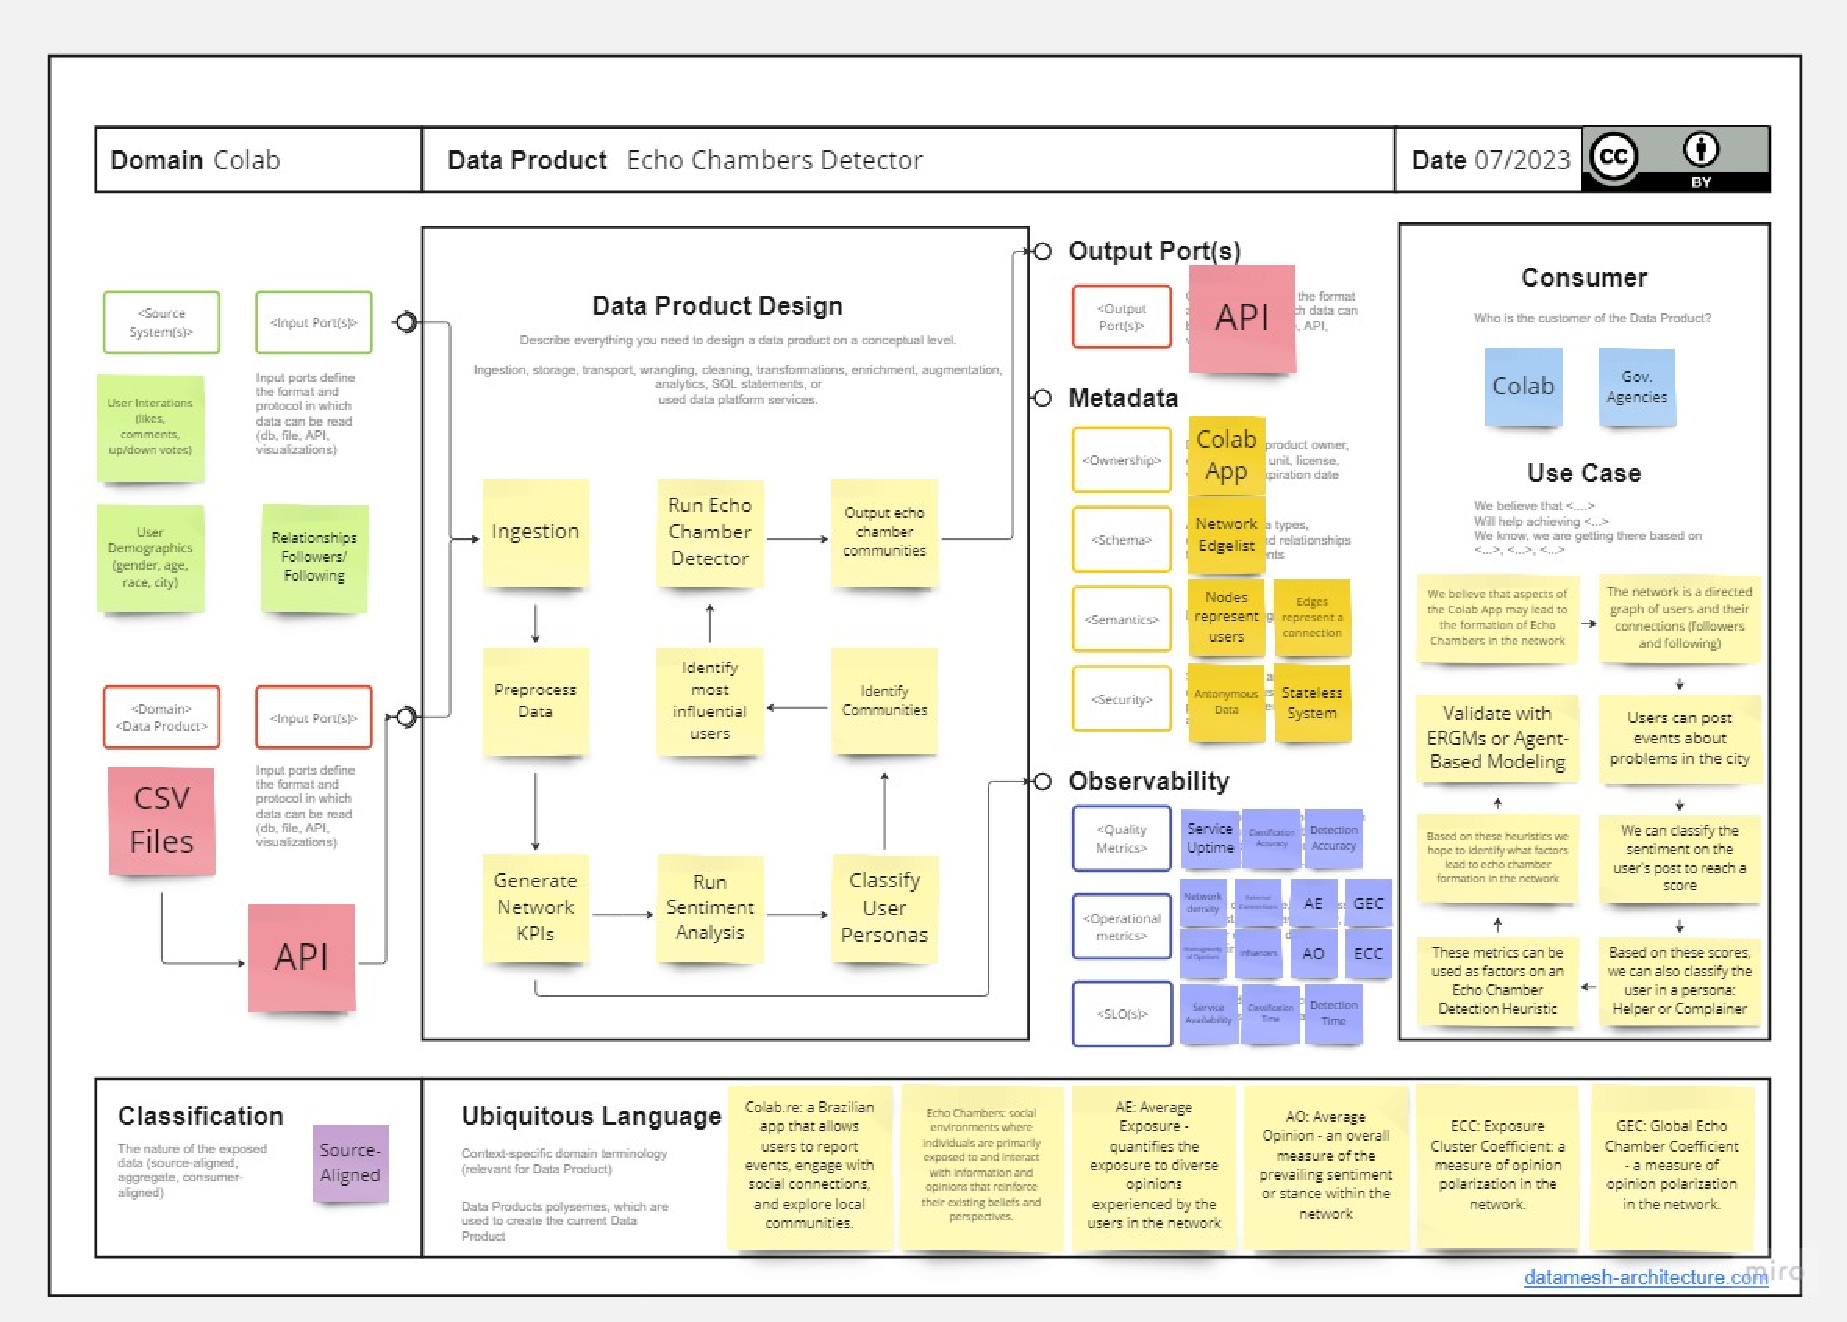
\includegraphics[scale=0.5]{tex/includes/data_canvas.pdf}
	\fautor
\end{figure}

Durante as discussões exploratórias com a equipe do Colab, elaboramos o Data Product Canvas como parte integrante da metodologia adotada para o desenvolvimento do aplicativo de detecção de câmaras de eco. O canvas proporcionou uma estrutura sólida e organizada para entendermos os requisitos do aplicativo e definirmos os diferentes elementos envolvidos em seu design e implementação.

Na seção de "Portos de Entrada", identificamos as interações dos usuários, como curtidas, comentários e votos positivos/negativos, juntamente com dados demográficos relevantes, como gênero, idade, raça e localidade. Além disso, consideramos as conexões entre usuários, representadas por seguidores e pessoas seguidas. Esses portos de entrada são fundamentais para a coleta dos dados necessários para análise e detecção de câmaras de eco na rede.

O design do produto de dados foi delineado em várias etapas, desde a ingestão dos dados até a geração de KPIs da rede, execução da análise de sentimentos, classificação das personas dos usuários, identificação de comunidades, detecção de usuários influentes, até a execução do detector de câmaras de eco e a saída das comunidades identificadas. Essa abordagem sequencial e bem definida permitirá uma análise abrangente e sistemática das câmaras de eco presentes na rede, fornecendo insights valiosos sobre sua formação e dinâmica.

Ao considerar os "Portos de Saída", optamos por utilizar uma API para disponibilizar as comunidades de câmaras de eco detectadas pelo aplicativo. Essa escolha nos permite fornecer acesso eficiente e acessível aos resultados obtidos, tanto para o próprio Colab App quanto para agências governamentais interessadas em entender e abordar a formação de câmaras de eco na rede.

A seção de "Metadados" do nosso canvas é particularmente relevante, pois aborda aspectos essenciais para a compreensão e governança adequada dos dados. Nesse contexto, especificamos que o aplicativo pertence ao Colab App e adotamos um esquema de dados baseado em uma lista de arestas da rede. A semântica do produto de dados é definida pelas entidades que representam os usuários e pelas conexões que representam as relações entre eles. Além disso, consideramos a segurança dos dados, garantindo que todas as informações coletadas sejam anônimas e que o sistema seja stateless.

A observabilidade é um aspecto crítico para garantir a qualidade e o desempenho do aplicativo. Nesse sentido, definimos métricas relevantes, como tempo de atividade do serviço, precisão da detecção, precisão da classificação, densidade da rede, conexões externas, homogeneidade de opiniões, influenciadores, opinião média, exposição média, coeficiente de agrupamento de exposição e coeficiente de câmaras de eco global. Essas métricas nos permitirão monitorar e avaliar o desempenho do aplicativo, bem como a eficácia da detecção de câmaras de eco na rede.

No contexto dos consumidores, identificamos o Colab App e agências governamentais como as partes interessadas em utilizar as comunidades de câmaras de eco detectadas. Esses consumidores poderão aproveitar os insights fornecidos pelo aplicativo para entender a formação das câmaras de eco e desenvolver estratégias eficazes para mitigar seus efeitos negativos.

Considerando o caso de uso do aplicativo, ressaltamos a crença de que certos aspectos do Colab App podem levar à formação de câmaras de eco na rede. Nesse contexto, o aplicativo foi projetado para permitir que os usuários postem eventos relacionados a problemas em suas cidades. Além disso, a análise de sentimentos é aplicada a essas postagens, fornecendo uma pontuação que permite classificar os usuários em personas. Essas métricas são fatores essenciais na heurística de detecção de câmaras de eco, que busca identificar quais fatores contribuem para a formação dessas câmaras. Por fim, planejamos validar nossos resultados utilizando modelos ERGMs (Exponential Random Graph Models) ou modelos baseados em agentes para confirmar a robustez das detecções feitas pelo aplicativo.

O uso do Data Product Canvas revelou-se essencial para estabelecer uma abordagem estruturada e colaborativa no desenvolvimento do aplicativo de detecção de câmaras de eco. Através desse framework, foi possível uma clara definição dos requisitos, elementos de design e aspectos operacionais do aplicativo, guiando todo o processo de desenvolvimento de forma sistemática.

Ao adotar o Data Product Canvas, buscamos não somente construir um aplicativo funcional, mas também obter uma compreensão aprofundada das dinâmicas de formação e impacto das câmaras de eco na rede do Colab App. Com uma definição clara dos portos de entrada, como as interações dos usuários e seus dados demográficos, e a utilização de técnicas de análise de sentimentos e classificação de personas, esperamos gerar insights valiosos para a mitigação dos efeitos negativos dessas câmaras.

Essa abordagem orientada pelo Data Product Canvas permite uma visão holística do aplicativo, contemplando desde a ingestão e pré-processamento dos dados até a identificação e classificação das comunidades de câmaras de eco. Com a identificação dos portos de saída, como uma API para disponibilizar as comunidades detectadas, buscamos assegurar a acessibilidade dos resultados tanto para os usuários do Colab App quanto para as agências governamentais interessadas.

Portanto, a aplicação do Data Product Canvas no desenvolvimento do aplicativo de detecção de câmaras de eco fortaleceu a estrutura do projeto, promovendo um processo colaborativo e possibilitando uma compreensão aprofundada das dinâmicas sociais envolvidas. Essa abordagem estruturada e integrada nos permite vislumbrar uma contribuição significativa para a identificação e mitigação das câmaras de eco no contexto do Colab App, fornecendo uma base sólida para a promoção de uma troca de informações mais diversificada e inclusiva na rede.

\section{Considerações Éticas e limitações}
Ao conduzir esta pesquisa, dedicamos especial atenção às considerações éticas e às questões de privacidade dos usuários. Todas as diretrizes éticas foram rigorosamente seguidas, e medidas foram adotadas para garantir a confidencialidade e o anonimato dos dados utilizados. Respeitamos a privacidade dos usuários do aplicativo Colab, tratando todas as informações de maneira sensível e em conformidade com as regulamentações e políticas de proteção de dados.

Obtivemos todas as autorizações necessárias para acessar e utilizar os dados relacionados aos usuários do aplicativo Colab, garantindo a legalidade e a conformidade com as diretrizes estabelecidas. Além disso, asseguramos que todas as informações sensíveis fossem tratadas com responsabilidade, adotando medidas de segurança adequadas para evitar qualquer divulgação não autorizada.

É importante ressaltar que todos os procedimentos adotados nesta pesquisa estão em conformidade com as diretrizes éticas estabelecidas pelo Comitê de Ética em Pesquisa de nossa instituição. O projeto foi submetido a uma análise minuciosa, considerando todos os aspectos éticos relacionados à coleta, análise e divulgação dos dados. A integridade e a validade dos resultados foram salvaguardadas por meio da adesão rigorosa às normas e regulamentos éticos.

Quanto às limitações do estudo, é válido destacar a natureza predominantemente quantitativa da pesquisa. Embora tenhamos empregado técnicas de análise de redes, algoritmos de agrupamento e detecção de comunidades, bem como a utilização de modelos epidemiológicos digitais, reconhecemos que uma abordagem exclusivamente quantitativa pode limitar a compreensão completa do fenômeno em estudo.

Para complementar a análise objetiva das interações dos usuários e a disseminação de informações nas câmaras de eco, é importante considerar abordagens qualitativas. Entrevistas e análise de conteúdo podem fornecer insights valiosos sobre as percepções, atitudes e motivações dos usuários envolvidos nas câmaras de eco. A combinação dessas abordagens quantitativas e qualitativas permitiria uma compreensão mais abrangente e rica do fenômeno.

É fundamental reconhecer e abordar as limitações inerentes a qualquer pesquisa, garantindo que os resultados sejam interpretados com cautela e considerando possíveis viéses ou lacunas no estudo. Ao fazê-lo, podemos avançar no conhecimento sobre as câmaras de eco no contexto do Colab App, contribuindo para uma compreensão mais completa desse fenômeno complexo e fornecendo subsídios para ações mitigadoras efetivas.

\section{Disponibilidade do Código-Fonte}
O código-fonte desenvolvido neste projeto está disponível em um repositório público no GitHub. Ele contém as implementações dos algoritmos de construção da rede social, algoritmos de agrupamento, modelos de epidemiologia digital e o desenvolvimento do painel em tempo real. O repositório pode ser acessado no seguinte endereço:\url{https://github.com/guinetik/colab-network-ec}.

\chapter{Uma Visão Geral do Colab.re}
\label{chapter:04_colab}
A participação cidadã e a colaboração por meio de empresas de tecnologia especializadas em negócios de governança pública, conhecidas como Gov-Techs,  têm se tornado cada vez mais relevantes na sociedade contemporânea. Com os avanços tecnológicos e a disseminação das redes sociais, surgiram novas formas de engajamento e interação entre cidadãos e governos. Nesse contexto, o aplicativo Colab se destaca como uma plataforma inovadora que combina elementos de redes sociais com a participação cidadã em questões relacionadas à gestão pública.

Neste capítulo, abordaremos o Colab a partir de uma perspectiva que envolve as redes sociais, e-Gov (governo eletrônico) e Gov-Techs, bem como a vigilância participativa. Analisaremos suas funcionalidades, impactos sociais, desafios e limitações, explorando o papel desempenhado pelo Colab nesse contexto dinâmico de engajamento cidadão e colaboração com as instâncias governamentais.

\section*{História e Desenvolvimento}
O Colab foi lançado em 2013 como uma iniciativa pioneira no campo da participação cidadã digital. A plataforma foi desenvolvida pelos sócios Paulo Pandolfi e Gustavo Maia, que, inspirados por suas experiências em marketing político, perceberam a necessidade de uma ferramenta que permitisse uma maior interação entre cidadãos e governos \cite{2023_Colab_PAGE}.

O objetivo do Colab é permitir que os usuários compartilhem ideias, façam sugestões, denunciem problemas e participem ativamente na construção de políticas públicas. Funcionando como uma rede social, os cidadãos podem postar fotos de problemas da cidade e solicitar uma solução. As prefeituras, por sua vez, acessam essas reclamações e têm uma solução de tecnologia em nuvem para dar andamento às solicitações \cite{2023_Colab_PAGE}.

Desde o seu lançamento, o Colab tem conquistado espaço em diversas cidades, tornando-se uma ferramenta de referência no campo da democracia digital. A plataforma foi eleita “o melhor app urbano do mundo” pela NewCities Foundation e hoje conta com 200 mil cadastros e contratos com diversas cidades, incluindo Recife, Ipojuca, Niterói, Mesquita, Maceió, Aracaju, Cruz Alta, Santo André e Juiz de Fora \cite{2023_Colab_PAGE}.

Além disso, desde 2016, o Colab também oferece uma ferramenta para que as prefeituras abram consultas sobre questões da cidade, auxiliando na tomada de decisões e na coleta de dados. Essa ferramenta tem vários formatos e gera muitos dados que ajudam a fazer uma gestão melhor com a participação do cidadão \cite{2023_Colab_PAGE}.

A história do Colab é marcada por desafios e inovações. Quando foi lançado, o aplicativo não tinha nenhuma prefeitura cadastrada. As necessidades dos cidadãos eram coletadas pela empresa e enviadas para a administração pública pelos canais de atendimento tradicionais, como site e email. No entanto, mesmo sem prefeituras cadastradas, o sistema foi reconhecido internacionalmente pela NewCities Foundation como "o melhor app urbano do mundo" \cite{2023_Colab_PAGE}.

A primeira prefeitura a adotar oficialmente o Colab foi Curitiba, seguida por outras 50 no mesmo ano. Esse crescimento rápido trouxe desafios, pois a empresa precisava atender melhor e evoluir, mas ainda não tinha receita. No entanto, um contrato com a organização social Comunitas, no começo de 2015, para atender as cidades de Santos e Campinas, em São Paulo, e Pelotas, no Rio Grande do Sul, injetou dinheiro na empresa e deu ânimo aos empreendedores \cite{2023_Colab_PAGE}.

Desde a sua fundação, o Colab tem buscado desenvolver soluções tecnológicas que possam contribuir para a construção de uma gestão pública mais eficiente, transparente e participativa. Atualmente, a plataforma está presente em mais de 130 cidades, em 2 países, e conta com cerca de 900 mil usuários cadastrados \cite{2023_Colab_PAGE}.

Hoje, a plataforma tem 200 mil cadastros e contratos com diversas cidades, incluindo Recife, Ipojuca, Niterói, Mesquita, Maceió, Aracaju, Cruz Alta, Santo André e Juiz de Fora. O valor dos contratos varia de 38 mil a 500 mil reais por ano, calculado com base na população da cidade e na quantidade de módulos contratados.

\section*{Funcionalidades}

\begin{figure}[!htb]
	\caption{Tela inicial do app Colab}
	\label{fig:colab_app}
	\centering
	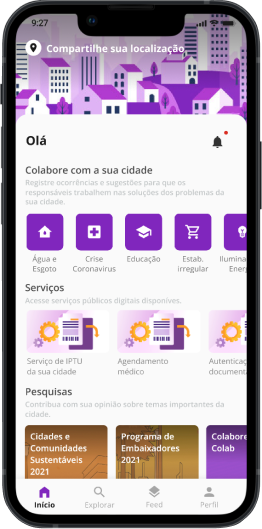
\includegraphics[scale=0.5]{colab_app.png}
\end{figure}

O Colab é uma plataforma digital que promove a vigilância participativa, a democracia digital e o governo eletrônico (e-Gov) por meio de uma série de funcionalidades interativas. A plataforma se destaca por permitir que os cidadãos desempenhem um papel ativo na gestão pública, contribuindo com ideias, sugestões e denúncias, e participando de consultas públicas.

A funcionalidade de publicação de ideias e sugestões permite que os usuários compartilhem suas ideias sobre questões de interesse público, abrangendo uma variedade de temas, desde melhorias na infraestrutura urbana até propostas de políticas sociais. Essa funcionalidade promove a democracia digital, permitindo que os cidadãos participem ativamente na formulação de políticas públicas.

A funcionalidade de denúncia de problemas permite que os usuários denunciem problemas como buracos nas vias, iluminação pública deficiente, entre outros. Essas denúncias são georreferenciadas, facilitando a identificação e resolução dos problemas pelas autoridades competentes. Isso contribui para a vigilância participativa, pois permite que os cidadãos monitorem a qualidade dos serviços públicos e infraestruturas em suas comunidades.

O Colab também possui uma forte componente social. Os usuários podem seguir outros usuários, serem seguidos, curtir e comentar as publicações. Isso promove a formação de uma rede social dentro do Colab, ampliando as possibilidades de engajamento e diálogo entre os participantes.

Os usuários também podem acompanhar o andamento das demandas e propostas que foram apresentadas. Isso permite que eles estejam cientes das ações tomadas pelo governo em resposta às suas contribuições, promovendo a transparência e a responsabilidade no governo eletrônico.

Além disso, o Colab introduziu recentemente novas funcionalidades, como micro consultas, reportar comentários e priorização de comentários. As micro consultas permitem que os usuários respondam perguntas rápidas do tipo sim/não diretamente na notificação push, trazendo mais dinamismo e velocidade para a gestão do relacionamento entre o cidadão e a cidade. A funcionalidade de reportar comentários permite que os usuários do Colab reportem comentários uns dos outros, mantendo a qualidade e a relevância das discussões na plataforma. A priorização de comentários, também conhecida como up/down vote, permite que os usuários indiquem o quão relevante um comentário é por meio de votos, destacando as contribuições mais valiosas.

A funcionalidade de consultas públicas é uma parte essencial do Colab, permitindo que os governos interajam diretamente com os cidadãos e obtenham feedback sobre várias questões. As consultas podem ser personalizadas para se adaptarem à realidade de cada território, e os gestores públicos podem criar seus próprios processos. Além disso, é possível configurar as consultas para permitir respostas anônimas. Essa funcionalidade promove a democracia digital e o governo eletrônico, permitindo que os cidadãos participem diretamente na tomada de decisões do governo.

A gamificação é um aspecto central do Colab, usada para aumentar o engajamento dos cidadãos e incentivá-los a participar ativamente na melhoria de suas cidades. A gamificação envolve o uso de elementos de design de jogos em contextos não-jogáveis para motivar a participação, envolvimento e lealdade.

No Colab, a gamificação é implementada através da "Jornada do Cidadão", uma trilha com desafios que orientam o cidadão sobre como ele pode colaborar e participar mais para tornar sua cidade melhor. Ao completar esses desafios, os cidadãos recebem recompensas e conquistas, que podem ser compartilhadas com outros usuários. Isso não apenas incentiva a participação contínua, mas também ajuda a disseminar uma cultura de participação dentro da cidade.

A gamificação no Colab não se limita apenas a incentivar a participação dos cidadãos. Ela também pode ser usada para conscientizar sobre determinadas causas ou estimular a participação em eventos. Por exemplo, se um hemocentro da cidade precisa de mais doações de sangue, a gestão pública pode criar um desafio no Colab para incentivar os cidadãos a doar sangue. Ao fazer isso, os cidadãos podem ganhar conquistas como "doador" ou "zelador do patrimônio público", reforçando a importância de suas contribuições para a cidade.

Em resumo, o Colab é uma plataforma que combina elementos de vigilância participativa, democracia digital e governo eletrônico para promover a participação cidadã na gestão pública. Através de suas diversas funcionalidades, o Colab busca fortalecer a participação cidadã, criar um ambiente propício para o diálogo entre cidadãos e governos, e promover a transparência e a responsabilidade no governo.

\section*{Gov Techs}
As gov techs são empresas que fornecem soluções tecnológicas para o setor público. Elas desempenham um papel crucial na modernização dos serviços governamentais, melhorando a eficiência, a transparência e a participação cidadã. Os serviços prestados ao governo por empresas de gov tech podem variar amplamente, dependendo das necessidades específicas do governo. Alguns exemplos incluem:

\begin{itemize}
	\item Digitalização de processos burocráticos: Isso pode incluir a criação de sistemas de gerenciamento de documentos, plataformas de pagamento online e sistemas de agendamento de compromissos.
	\item Plataformas de participação cidadã: Estas são plataformas que permitem aos cidadãos participar diretamente na tomada de decisões do governo. Isso pode incluir a votação em questões políticas, a apresentação de propostas de políticas e a participação em discussões públicas.
	\item Soluções de análise de dados: As empresas de gov-tech podem fornecer soluções que ajudam o governo a coletar, analisar e interpretar grandes quantidades de dados. Isso pode ajudar o governo a tomar decisões mais informadas e eficazes.
\end{itemize}

O Colab é um exemplo de uma solução de gov tech que se destaca na indústria pelo seu aspecto social. Como uma plataforma de participação cidadã, o Colab permite que os cidadãos se envolvam diretamente na tomada de decisões do governo, promovendo a transparência e a responsabilidade. Isso representa uma mudança significativa na forma como o governo interage com os cidadãos, permitindo uma maior inclusão e participação na tomada de decisões.

No entanto, a adoção de soluções de gov tech como o Colab não está isenta de desafios. De acordo com um estudo de \citeonline{2021_Liang}, fatores como a competência do provedor, a prontidão organizacional, a pressão externa e a confiança na tecnologia desempenham um papel significativo na adoção de tecnologias de nuvem móvel no governo. Esses fatores podem ser igualmente aplicáveis ao Colab e outras soluções de gov tech, e precisam ser considerados cuidadosamente ao implementar essas tecnologias.

Além disso, a tecnologia blockchain está emergindo como uma nova ferramenta potencial para o setor público. \citeonline{2021_Diakiv} identifica dez direções potenciais para o uso de tecnologias blockchain no setor público, incluindo autenticação, rastreabilidade e singularidade. Embora o Colab não utilize a tecnologia blockchain, a crescente importância dessa tecnologia no setor público sugere que pode ser uma área para futura exploração ou integração.

Finalmente, a ética na tecnologia é uma consideração importante na adoção de soluções de gov tech. \citeonline{2022_Grellette} sugere a realização de auditorias de confiança como uma maneira de melhorar a prática da ética na tecnologia. Isso poderia ser relevante para o Colab e outras soluções de gov tech, à medida que buscam ganhar e manter a confiança do público.

\section*{Interfaces para problemas urbanos}
Devido a adoção em massa de aplicativos e a alta disponibilidade da internet, softwares sociais e de vigilância participativa tem se tornado interfaces para problemas urbanos. Essas interfaces têm desempenhado um papel crucial na resolução de questões relacionadas às cidades. Vários estudos de caso têm evidenciado a eficácia dessa ferramenta em abordar desafios urbanos e promover a participação cidadã.

\citeonline{2021_Barros} avaliaram o Colab juntamente com outras duas iniciativas de democracia digital, Mudamos e Panela de Pressão. A avaliação considerou diferentes aspectos, como recursos tecnológicos, modos de participação online, atores envolvidos, objetivos políticos das iniciativas e captação de recursos. Os resultados destacaram a importância da estrutura organizacional na compreensão do desenvolvimento bem-sucedido de iniciativas de democracia digital.

\citeonline{2015_Silva} analisaram o Colab como uma ferramenta de colaboração e mobilidade urbana. Esse estudo ressaltou a relevância do Colab como uma plataforma que permite aos cidadãos participarem ativamente da melhoria de suas cidades, fornecendo um canal direto de feedback às autoridades municipais sobre problemas urbanos.

O estudo de \citeonline{2018_CARVALHO_DISSERTATION} explora o uso do aplicativo móvel Colab.re para promover a participação social na gestão da cidade de Paragominas, no estado do Pará, Brasil. Apesar de Paragominas ser uma cidade relativamente isolada, o estudo demonstrou que a implementação do Colab.re resultou em um canal eficaz de comunicação entre a prefeitura e os cidadãos, alcançando o maior percentual de usuários do aplicativo em todo o estado do Pará. As conclusões de Carvalho indicam que a Computação Urbana e o uso de dispositivos móveis podem fortalecer as relações entre os usuários e ajudar a entender melhor como os problemas pontuais afetam a cidade como um todo. O estudo destaca o potencial da Computação Urbana e de aplicativos móveis para melhorar a gestão das cidades, promovendo a participação social e melhorando a comunicação entre os cidadãos e as autoridades municipais, mesmo em áreas isoladas como Paragominas.

Esses estudos de caso fornecem evidências concretas de como o Colab tem sido uma interface valiosa na resolução de problemas urbanos. Sua capacidade de promover a participação cidadã, coletar feedback dos cidadãos e melhorar a prestação de serviços públicos o torna uma ferramenta relevante para impulsionar mudanças positivas nas cidades. Através do Colab e de outras interfaces similares, é possível fortalecer a colaboração entre os cidadãos, autoridades municipais e outros atores envolvidos na busca por soluções inovadoras e sustentáveis para os desafios urbanos.

\section*{Engajamento Cidadão e Plataformas Digitais na Era da COVID-19}
A pandemia de COVID-19 apresentou desafios sem precedentes para a participação cidadã e o engajamento social. Em resposta a esses desafios, plataformas digitais emergiram como ferramentas vitais para facilitar a participação cidadã na gestão pública, mesmo em meio ao distanciamento social.

\subsection*{Vigilância Participativa}
A vigilância participativa é uma abordagem inovadora que envolve o engajamento ativo da comunidade no processo de coleta, monitoramento e compartilhamento de informações relevantes para identificar e responder a problemas sociais, ambientais e de saúde. 

\begin{citacao}
	"uma forma de inteligência coletiva em que as pessoas se reúnem para monitorar, analisar e agir coletivamente em relação a um problema ou questão compartilhada" \cite[p. 1]{2011_Bryer}.
\end{citacao}

Com os avanços tecnológicos e a disseminação de dispositivos móveis e plataformas digitais, a aplicação de aplicativos móveis para a vigilância participativa tem ganhado destaque. Nesta seção, exploramos o conceito de vigilância participativa, apresentando sua definição e abordando sua relevância no contexto atual.

A vigilância participativa tem sido reconhecida como uma abordagem promissora para a coleta de informações em tempo real, permitindo que a comunidade desempenhe um papel ativo na detecção e monitoramento de problemas sociais, ambientais e de saúde. Tradicionalmente, a vigilância tem sido realizada por meio de sistemas centralizados e conduzida por especialistas em saúde ou autoridades governamentais. No entanto, com a proliferação de dispositivos móveis, o acesso à internet e o surgimento de plataformas colaborativas, os aplicativos móveis têm sido adotados como ferramentas eficazes para engajar os cidadãos na vigilância participativa.

O conceito de vigilância participativa foi formalmente reconhecido pelas Regulamentações Sanitárias Internacionais (RSIs) revisadas em 2005, as quais ampliaram o escopo da vigilância além dos mecanismos tradicionais. Esse reconhecimento proporcionou uma oportunidade para a integração de canais não oficiais e melhorias tecnológicas para agilizar a detecção, o monitoramento e a resposta a problemas de saúde. A vigilância participativa utiliza métodos de crowdsourcing para coletar informações da sociedade e devolver o conhecimento coletivo de volta à comunidade.\cite[1]{2017_Smolinski}

Um estudo de caso relevante que exemplifica a aplicação da vigilância participativa é a iniciativa "Saúde na Copa" durante a Copa do Mundo FIFA de 2014, realizada no Brasil. O projeto utilizou um aplicativo de vigilância participativa chamado Healthy Cup, permitindo que usuários de todo o mundo relatassem suas condições de saúde em tempo real. Ao focar em três síndromes específicas e seis doenças relevantes para aglomerações de pessoas, o aplicativo facilitou a detecção precoce de surtos de doenças agudas ao identificar agregados de sintomas indicativos de doenças infecciosas \cite{2017_LealNeto}.

Além da saúde, a vigilância participativa também tem sido aplicada em outras áreas, proporcionando benefícios semelhantes e promovendo a participação ativa da comunidade. Essa abordagem colaborativa tem se mostrado útil na vigilância de diversos aspectos do ambiente e da sociedade, permitindo que os cidadãos desempenhem um papel ativo na coleta e compartilhamento de informações relevantes.

Um exemplo notável é o uso da vigilância participativa na monitorização da qualidade do ar por meio do aplicativo AirVisual. Com a contribuição dos usuários, juntamente com dados oficiais de estações de monitoramento, é possível mapear e identificar áreas com problemas de poluição atmosférica. Os cidadãos podem relatar os níveis de poluição do ar em suas áreas, fornecendo informações valiosas para a vigilância participativa desse aspecto crucial do ambiente. Essa abordagem empodera os indivíduos a agirem como agentes ativos na identificação de áreas com poluição do ar significativa, contribuindo para a tomada de decisões informadas e para a melhoria da qualidade do ar nas comunidades.

\begin{figure}[!htb]
    \caption{Aplicativo NoiseTube exibindo o nível de ruído em uma localidade}
    \label{fig:app_noisetube}
    \centering
    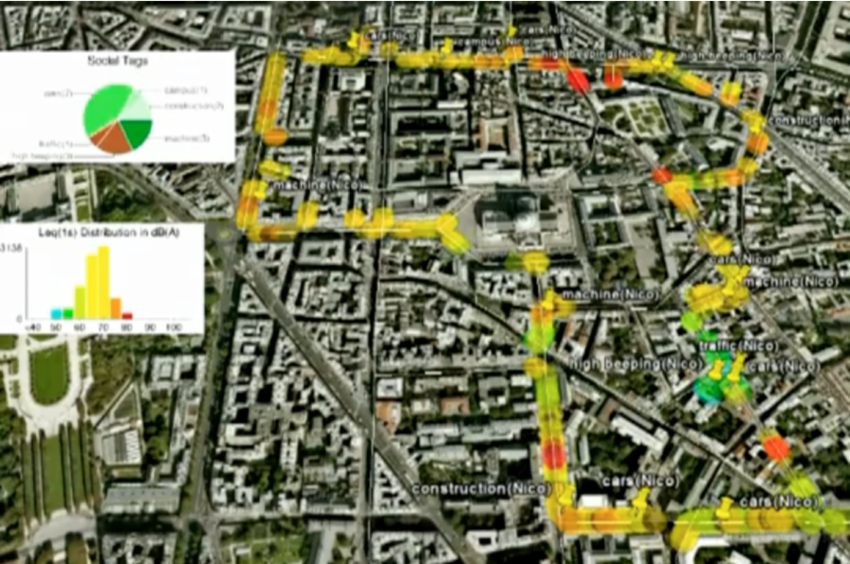
\includegraphics[scale=0.8]{app_noisetube.png}
    \fdireta{2010_Arnand}
\end{figure}

Outra área em que a vigilância participativa tem desempenhado um papel importante é a monitorização do ruído ambiental. O aplicativo NoiseTube permite que os usuários realizem medições de ruído e compartilhem esses dados, criando um mapa colaborativo do ruído em diferentes localidades. Essa vigilância participativa do ruído ambiental permite a identificação de áreas com altos níveis de ruído, auxiliando na tomada de medidas para mitigar os efeitos adversos na saúde e no bem-estar da comunidade. Ao participar ativamente da vigilância do ruído, os cidadãos contribuem para a criação de ambientes mais saudáveis e para a implementação de políticas públicas adequadas \cite{2010_Arnand}.

Esses exemplos ilustram como a vigilância participativa pode ser aplicada em diferentes áreas, além da saúde. Ao envolver os cidadãos na coleta e compartilhamento de informações relevantes, a vigilância participativa se torna uma ferramenta poderosa para a identificação e resposta a problemas ambientais e sociais. Essa abordagem colaborativa, combinada com o uso de tecnologias móveis e plataformas digitais, fortalece a relação entre a comunidade e as autoridades responsáveis, promovendo uma governança mais inclusiva e eficaz.

\subsection*{Iniciativa Brasil Sem Corona}

A Iniciativa Brasil Sem Corona, uma colaboração entre o Colab e a startup Epitrack, exemplifica o uso eficaz da tecnologia para facilitar a participação cidadã durante uma crise de saúde pública. Através desta iniciativa, os dados sobre a pandemia de COVID-19 foram coletados diretamente dos cidadãos, que relataram seus sintomas e receberam informações sobre como se proteger do vírus. Esses dados foram então utilizados para gerar mapas de calor que auxiliaram as autoridades de saúde a identificar e responder a surtos de COVID-19.

Na cidade de Caruaru/PE, a iniciativa teve resultados significativos. O projeto contou com 861 usuários ativos, apresentando uma média de 1,2 relatórios por usuário por semana. A plataforma Brasil Sem Corona começou em 20 de março e, desde então, tem sido oficialmente utilizada pela autoridade de saúde de Caruaru para melhorar a qualidade das informações do sistema de vigilância tradicional. Em relação aos casos de síndrome respiratória do sistema de vigilância tradicional, 1.588 indivíduos foram positivos para este resultado clínico. A análise de varredura espacial detectou 18 aglomerados e 6 deles apresentaram significância estatística (valor p < 0,1). Os aglomerados 3 e 4 apresentaram uma área de sobreposição que foi escolhida pela autoridade local para implantar a sorologia de Covid-19, onde 50 indivíduos foram testados. Desses, 32\% (n=16) apresentaram resultados reagentes para anticorpos relacionados à Covid-19 \cite[1]{2020_LealNeto}. Essa pesquisa demonstra como a vigilância participativa pode ser uma ferramenta eficaz para melhorar a qualidade das informações do sistema de vigilância tradicional, permitindo uma detecção precoce de surtos de COVID-19 e uma resposta mais eficaz, principalmente quando aliado a uma aplicação de alta disponibilidade e adoção pela população.

\section{Reflexões sobre o Colab}

As soluções de empresas Gov Tech têm emergido como catalisadores poderosos na transformação das relações entre cidadãos e órgãos governamentais. Estas plataformas, como o Colab, não apenas facilitam a comunicação, mas também redefinem a dinâmica da participação cidadã, tornando-a mais direta, transparente e, sobretudo, democrática. No entanto, a mesma interconexão que possibilita essa participação ampliada também pode criar ambientes isolados, as chamadas câmaras de eco, onde os usuários são frequentemente expostos apenas a opiniões que reforçam suas crenças preexistentes.

O Colab, ao promover a participação ativa e informada dos cidadãos, tem o potencial de contrabalançar os efeitos negativos das câmaras de eco. Ao incentivar o diálogo aberto e a colaboração entre cidadãos de diferentes backgrounds e perspectivas, a plataforma pode ajudar a criar uma sociedade mais informada e resiliente. Através da análise dos perfis dos usuários e das postagens, foi possível identificar tendências, prioridades e problemas recorrentes, fornecendo subsídios importantes para a formulação de políticas públicas mais eficazes e direcionadas.

A diversidade de gênero e a representatividade na participação cívica são fundamentais para garantir uma governança inclusiva e representativa. A combinação de abordagens digitais e tradicionais pode gerar resultados mais abrangentes e inclusivos, evitando a exclusão digital e garantindo a participação de todos os segmentos da sociedade.

No entanto, é fundamental que as plataformas sejam projetadas levando em consideração a usabilidade, a acessibilidade e a segurança dos dados dos usuários. Políticas claras de privacidade e proteção de dados devem ser implementadas, garantindo a confidencialidade das informações compartilhadas e a confiança dos usuários na plataforma.

Em um mundo cada vez mais digital, onde as câmaras de eco podem distorcer a percepção da realidade e influenciar decisões, plataformas como o Colab surgem como ferramentas essenciais para garantir que a voz do cidadão seja ouvida, respeitada e incorporada nas políticas públicas. Ao explorar o potencial das plataformas de engajamento cívico, os governos podem fortalecer a democracia, criar comunidades mais participativas e resilientes e, sobretudo, garantir que as decisões tomadas reflitam verdadeiramente as necessidades e desejos da população.

\section{Fonte de Dados}
Nesta pesquisa, utilizamos como fonte de dados o conjunto de informações coletadas e disponibilizadas pela equipe de R\&D do Colab. Esses dados consistem em listas de arestas, que representam as conexões entre os usuários,suas interações como likes e comentários, e suas postagens realizadas entre os anos de 2016 e 2022. Limitamos alguns aspectos da pesquisa às cidades de Caruaru, Rio de Janeiro, Recife, Niterói, Mesquita e Santo André, a fim de obter uma amostra representativa dessas regiões.

A coleta dos dados foi possível através de parcerias estabelecidas com a equipe do Colab, que nos concedeu acesso ao conjunto de informações. Esses dados são de grande relevância para o desenvolvimento da pesquisa, pois nos permitem examinar as interações sociais e os padrões de engajamento dos usuários dentro da plataforma.

\subsection*{Modelo de dados}
\label{sec:modelo_de_dados}

Os dados dos foram disponibilizados em formato CSV, contendo informações sobre os usuários e os eventos reportados. A seguir, é apresentado um resumo mo modelo de dados utilizados:

\begin{itemize}
	\item User (\autoref{tab:user_model}): Dados dos usuários
	\item Connection (\autoref{tab:connections_model}): Conexão entre os usuários, com lista de seguidores/seguindo.
	\item Events (\autoref{tab:event_model}): Eventos reportados pelos usuários.
	\item Likes (\autoref{tab:interactions_model}): Apoios/curtidas na rede social.
	\item Comments (\autoref{tab:interactions_model}): Comentários em publicações de outros usuários.
	\item UpDown Vote (\autoref{tab:updown_model}): Endosso ou rejeição a comentários de outros usuários.
\end{itemize}

\begin{table}[ht]
	\centering
	\caption{Tabela Users: Representa os usuários do app}
	\label{tab:user_model}
	\begin{tabularx}{\textwidth}{|l|X|}
		\hline
		\textbf{Campo}     & \textbf{Descrição}                              \\
		\hline
		colab\_user\_id    & Identificador único do usuário no app Colab 	 \\
		gender             & Gênero do usuário                               \\
		race               & Raça do usuário                               	 \\
		education          & Escolaridade do usuário                         \\
		birth\_date        & Data de nascimento do usuário                   \\
		city\_id           & Identificador único da cidade do usuário        \\
		city\_name         & Nome da cidade do usuário                       \\
		state\_id          & Identificador único do estado do usuário        \\
		state\_name        & Nome do estado do usuário                       \\
		created\_at        & Data de criação do registro do usuário          \\
		last\_sign\_in\_at & Data da última vez que o usuário fez login      \\
		device             & Dispositivo utilizado pelo usuário              \\
		\hline
	\end{tabularx}
\end{table}

\begin{table}[ht]
	\centering
	\caption{Tabela Connetion: Representa a conexão entre os usuários}
	\label{tab:connections_model}
	\begin{tabularx}{\textwidth}{|l|X|}
		\hline
		\textbf{Campo}    & \textbf{Descrição}                                   \\
		\hline
		source         	  & Identificador único do evento                        \\
		target            & Identificador único do usuário relacionado ao evento \\
		created\_at       & Data de criação, representando um follow             \\
		deleted\_at       & Data de deleção, representando um unfollow			 \\
		\hline
	\end{tabularx}
\end{table}

\begin{table}[ht]
	\centering
	\caption{Tabela Events: Representa os eventos reportados pelos usuários}
	\label{tab:event_model}
	\begin{tabularx}{\textwidth}{|l|X|}
		\hline
		\textbf{Campo}    & \textbf{Descrição}                                   \\
		\hline
		event\_id         & Identificador único do evento                        \\
		user\_id          & Identificador único do usuário relacionado ao evento \\
		description       & Descrição do evento                                  \\
		status            & Status do evento                                     \\
		created\_at       & Data de criação do evento                            \\
		event\_type\_id   & Identificador único do tipo de evento                \\
		event\_type\_name & Nome do tipo de evento                               \\
		\hline
	\end{tabularx}
\end{table}

\begin{table}[ht]
	\centering
	\caption{Tabela Interactions: Representa as interações entre os usuários}
	\label{tab:interactions_model}
	\begin{tabularx}{\textwidth}{|l|X|}
		\hline
		\textbf{Campo}    & \textbf{Descrição}                                   		 		\\
		\hline
		user\_from        & O colab\_user\_id do usuário criador da curtida/apoio          		\\
		user\_to          & O colab\_user\_id do usuário recebidor da curtida/apoio  		 	\\
		created\_at       & Data de criação da interação        				 				\\
		\hline
	\end{tabularx}
\end{table}

\begin{table}[ht]
	\centering
	\caption{Tabela Up-Down Vote: Representa os endossos e rejeições de comentários}
	\label{tab:updown_model}
	\begin{tabularx}{\textwidth}{|l|X|}
		\hline
		\textbf{Campo}    & \textbf{Descrição}                                   		 		\\
		\hline
		user\_from        & O colab\_user\_id do usuário criador da curtida/apoio          		\\
		user\_to          & O colab\_user\_id do usuário recebidor da curtida/apoio  		 	\\
		rating            & Representa se o endosso foi Positivo/Up (1) ou Negativo/Down (0)  	\\
		created\_at       & Data de criação da interação           				 				\\
		\hline
	\end{tabularx}
\end{table}

A partir desses dados, criamos uma representação abrangente do ambiente social e das interações dos usuários dentro do aplicativo Colab. Utilizando o conjunto de informações coletadas, realizamos uma análise exploratória para compreender os padrões e comportamentos dos usuários. Apresentamos uma análise exploratória desses dados no \autoref{chapter:04_colab}.

\section{Análise exploratória dos dados}
\label{sec:colab_data_analysis}

Com base nos dados disponibilizados pelo Colab para esse estudo, analisamos um total de 328.876 eventos criados entre 04/01/2013 e 05/12/2022.

\subsection*{Distribuição demográfica}

O quadro \autoref{quadro:usersbygender} apresenta a distribuição demográfica dos usuários por gênero. A maioria dos usuários se declararam do gênero másculino.

\begin{quadro}[htb]
	\caption{Usuários por gênero}
	\label{quadro:usersbygender}
	\centering
	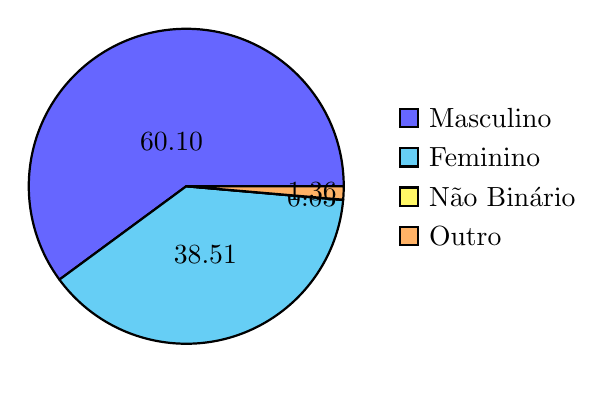
\begin{tikzpicture}
		\pie[
			sum=auto,
			text=legend,
			radius=2
		]{
			60.10/Masculino,
			38.51/Feminino,
			0.03/Não Binário,
			1.36/Outro/Desconhecido
		}
	\end{tikzpicture}
	\begin{tabular}{|l|r|}
		\hline
		\textbf{Gênero} & \textbf{Quantidade} \\
		\hline
		Masculino       & 30494               \\
		Feminino        & 19555               \\
		Não Binário     & 16                  \\
		Desconhecido    & 335                 \\
		Outro           & 274                 \\
		Não Informado   & 92                  \\
		\hline
	\end{tabular}
\end{quadro}

\subsection*{Tipos de Eventos}

\begin{table}[h]
	\centering
	\caption{Tipos de eventos com mais ocorrências}
	\label{tab:tiposevento}
	\begin{tabularx}{\textwidth}{|X|l|l|}
		\hline
		\textbf{Tipo de Evento}                  & \textbf{Total de Ocorrências} \\
		\hline
		Entulho na calçada/via pública           & 61.785                        \\
		Buraco nas vias                          & 41.200                        \\
		Lâmpada apagada à noite                  & 32.907                        \\
		Ponto de infração de trânsito recorrente & 15.873                        \\
		Calçada irregular                        & 14.837                        \\
		Mato alto                                & 13.459                        \\
		Poda de árvore                           & 12.810                        \\
		Descarte irregular de lixo               & 12.685                        \\
		Bueiro entupido                          & 8.825                         \\
		Vazamento de água                        & 7.433                         \\
		Bueiro sem tampa                         & 5.844                         \\
		Ocupação irregular de área pública       & 5.714                         \\
		Fiação irregular                         & 5.643                         \\
		Veículo abandonado                       & 5.335                         \\
		Equipamento público danificado           & 4.694                         \\
		Esgoto a céu aberto                      & 4.656                         \\
		Retirada de árvore                       & 4.437                         \\
		Ponto recorrente de poluição sonora      & 4.189                         \\
		Bloqueio na via                          & 4.066                         \\
		Iluminação pública irregular             & 3.702                         \\
		\hline
	\end{tabularx}
\end{table}

A tabela \autoref{tab:tiposevento} apresenta os 20 tipos de evento mais reportados pelos usuários. A análise dos dados fornecidos pelos usuários do Colab proporcionou insights valiosos sobre as preocupações e demandas da comunidade. Os eventos mais frequentemente relatados estão intrinsecamente ligados a problemas e irregularidades na infraestrutura urbana, como entulho na calçada/via pública, buraco nas vias, lâmpada apagada à noite, ponto de infração de trânsito recorrente e calçada irregular. Essas ocorrências destacam a importância de investimentos contínuos na manutenção e melhoria da infraestrutura da cidade. Além disso, questões ambientais emergem como uma área de preocupação significativa, com denúncias frequentes de descarte irregular de lixo, desmatamento ilegal, esgoto a céu aberto e mato alto. Essas postagens indicam uma conscientização dos usuários em relação à preservação ambiental e ressaltam a necessidade de ações efetivas para aprimorar a gestão dos recursos naturais. O transporte público também é alvo de atenção, com reclamações recorrentes sobre problemas em ônibus, atrasos e superlotação. Esses aspectos exigem uma análise aprofundada das questões relacionadas à mobilidade urbana e podem impulsionar esforços para melhorar a qualidade e eficiência do transporte coletivo. Eventos relacionados à segurança e vigilância, como pontos de exploração sexual de menores e maus-tratos a animais, refletem a preocupação dos usuários com a proteção e bem-estar da comunidade. A ocorrência de eventos envolvendo estabelecimentos comerciais, como falta de alvará e condições sanitárias irregulares, destaca a importância de ações rigorosas de fiscalização e de garantir a conformidade legal por parte dos estabelecimentos. Esses insights fornecem uma visão abrangente das preocupações dos usuários do Colab e podem orientar as prefeituras da cidade na implementação de políticas públicas que visem atender às demandas da comunidade e aprimorar a qualidade de vida em geral.

Os usuários estão engajados e ativos na identificação e denúncia de problemas na infraestrutura urbana, meio ambiente, transporte público e questões sociais. Isso indica uma participação cidadã ativa e um desejo de melhorar as condições de suas comunidades. Os clientes podem aproveitar essas informações para acompanhar as preocupações e demandas da comunidade, tomar medidas corretivas mais efetivas e aprimorar a qualidade dos serviços e infraestrutura oferecidos.

Os dados fornecem uma visão clara das principais questões enfrentadas pela comunidade, permitindo que as prefeituras priorizem recursos e esforços em áreas críticas, como manutenção da infraestrutura, gestão ambiental, transporte público e segurança. As prefeituras podem usar esses insights para desenvolver políticas públicas mais eficazes, implementar medidas preventivas e corretivas, bem como estabelecer canais de comunicação e interação mais robustos com os cidadãos, fortalecendo a confiança e a participação da comunidade nas decisões governamentais.

\subsection*{Frequência de postagens e engajamento}
\label{sec:engajamento}

\begin{quadro}[htb]
	\caption{Histograma demonstrando a distribuição de novos eventos por ano}
	\label{quadro:colab_events_overtime}
	\centering
	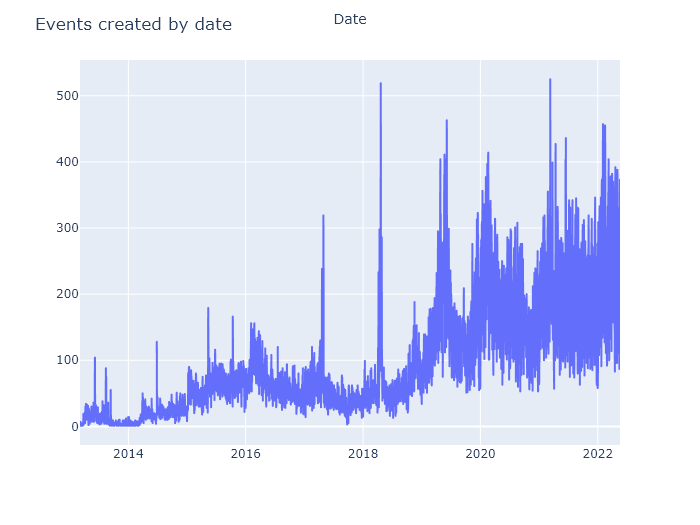
\includegraphics[scale=0.4]{colab_events_overtime.png}
\end{quadro}

O \autoref{quadro:colab_events_overtime} demonstra a criação de eventos ao longo dos anos. Na imagem pode-se identificar dois picos de mais de 500 postagens por mês: Abril de 2018 e Março de 2022. Além desses picos, é possível observar uma tendência geral de crescimento no número de postagens ao longo dos anos, com algumas flutuações. Por exemplo, em 2017, o número médio de postagens por mês foi de 231, enquanto em 2022, esse número aumentou para uma média de 389 postagens por mês. Isso sugere um aumento no engajamento dos usuários com o aplicativo Colab ao longo do tempo.

Também é interessante notar que o número de postagens tende a aumentar no início do ano, com picos observados em março de cada ano. Isso pode ser devido a fatores sazonais, como o aumento das chuvas no início do ano, que podem levar a mais problemas de infraestrutura urbana sendo relatados.

Em uma análise comparativa dos quatro tipos de interação analisados, observa-se que alguns estão em ascensão, enquanto outros apresentam diminuição na participação. Com o decorrer dos meses, há um aumento no número de curtidas e comentários. Existe uma forte correlação positiva entre a quantidade dessas interações e o tempo decorrido (0,80 para comentários e 0,62 para curtidas). No entanto, o mesmo não ocorre com as conexões e os votos positivos ou negativos nos comentários, que demonstram uma tendência de diminuição no uso. Seria interessante aprofundar a investigação para compreender o motivo dessa queda, especialmente nas conexões, a partir de julho de 2020.

\subsection*{Conexões}

Analisando-se as principais informações sobre a conectividade entre os usuários, isto é, o vínculo entre seguidores e as pessoas que os usuários estão seguindo, tem-se um total de 416.115 ligações. Dentre essas, 402.221 estão ativas e não foram desfeitas (deixar de seguir). As conexões ativas envolvem 112.699 usuários distintos, resultando em uma média de 4,2 conexões e uma mediana de 1 conexão por pessoa. Quanto ao número de seguidores, há variações entre 0 e 854, enquanto o número de pessoas seguidas pelos usuários varia entre 0 e 9.340.

\begin{figure}[!htb]
	\caption{Distribuição das conexões entre os usuários}
	\label{fig:colab_users_by_connection}
	\centering
	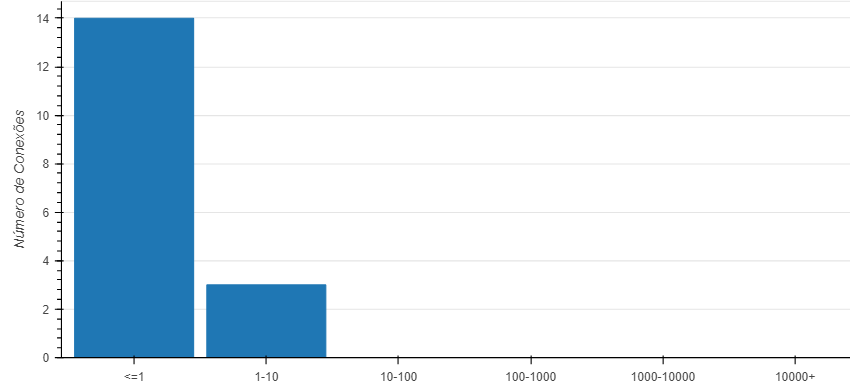
\includegraphics[scale=0.5]{images/colab_users_by_connection.png}
\end{figure}

Percebe-se que cerca de 83\% dos usuários possuem até 10 conexões, considerando-se a soma de seguidores e pessoas seguidas. Esse valor pode parecer baixo em comparação com outras redes sociais mais populares. No entanto, é importante ressaltar que cada plataforma possui suas particularidades e caberia aprofundar, em estudos futuros, a principal motivação dos usuários para estabelecerem conexões entre si. É possível que muitos usuários busquem se conectar com pessoas conhecidas em seu cotidiano, mas também pode haver usuários que possuam maior influência devido ao seu perfil de uso do aplicativo, por exemplo. Para compreender se há variações nos perfis de conexões em cada cidade, foram destacadas as informações de Mesquita, Niterói e Santo André.

De maneira geral, Niterói e Santo André apresentam comportamentos semelhantes, com melhor distribuição dos usuários nas faixas de 2-10 e 10-1000 conexões. Nessa última faixa, Niterói possui o maior percentual, com 14\%. Por outro lado, em Mesquita, prevalece a faixa de 1 conexão por usuário (53\%), o que pode indicar uma rede menos integrada (pelo menos em relação às conexões).

\begin{figure}[!htb]
	\caption{Distribuição das conexões entre os usuários de Mesquita, Niterói e Santo André}
	\label{fig:colab_users_by_connections_on_cities}
	\centering
	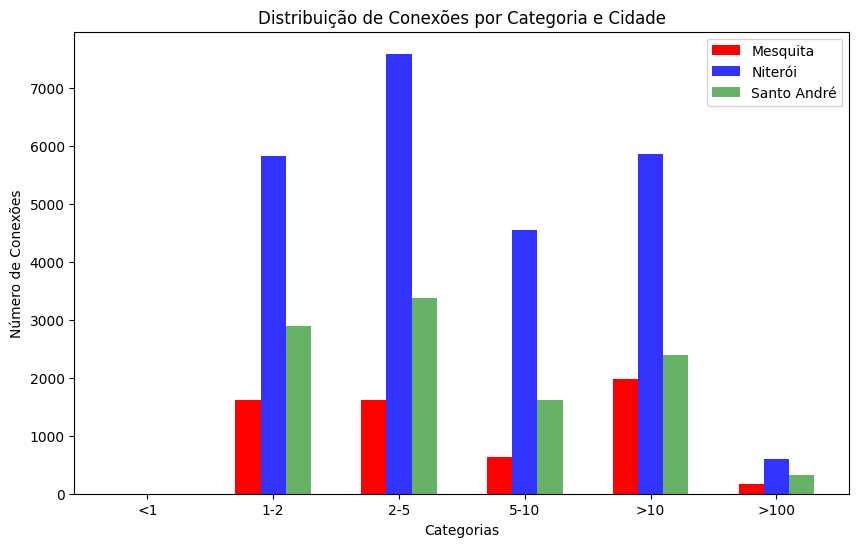
\includegraphics[scale=0.5]{images/colab_users_by_connections_on_cities.png}
\end{figure}

\subsection*{Apoios}

As curtidas no Colab são divididas em três grandes grupos: curtidas em publicações, comuniques ou propostas (que não existem mais). A plataforma conta com aproximadamente 1,5 milhão de curtidas, realizadas por um total de 100.265 usuários. Verifica-se que a maior parte das curtidas ocorre em publicações relacionadas à zeladoria, as quais representam o maior volume de atividades no feed. Em resumo, a média de curtidas por usuário é de 14, com uma mediana de 2 curtidas. Ao aprofundar a análise para o nível individual dos usuários, é possível constatar diferentes perfis, que variam de 1 até 51.966 curtidas. Apesar de alguns usuários apresentarem um comportamento discrepante, 85\% dos cidadãos realizaram até 10 curtidas. Ao analisar a participação nas três cidades selecionadas - Mesquita, Niterói e Santo André, não foram encontradas diferenças relevantes no percentual de curtidas.

\begin{figure}[!htb]
	\caption{Distribuição de curtidas ao longo dos anos}
	\label{fig:colab_likes_overtime}
	\centering
	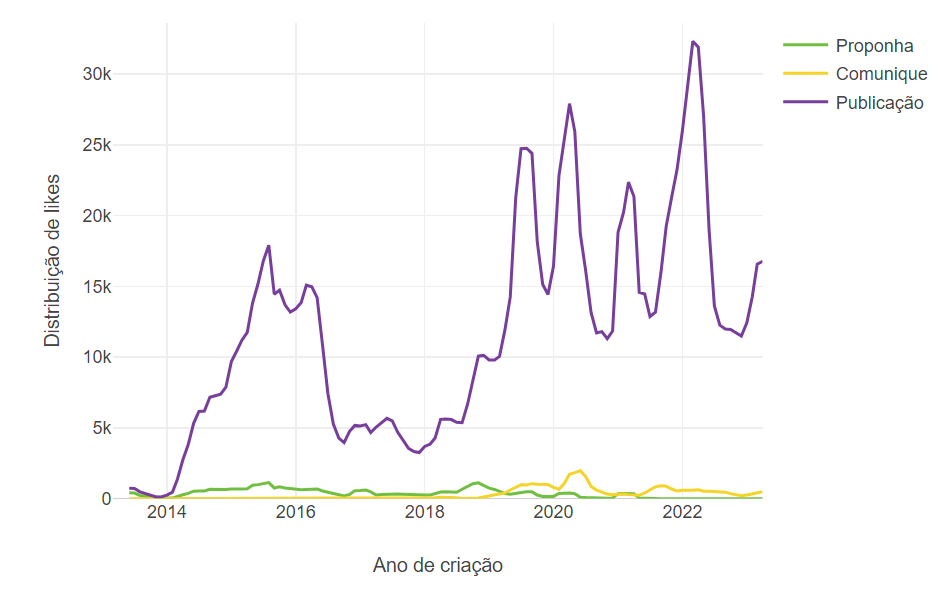
\includegraphics[scale=0.5]{images/colab_likes_overtime.png}
\end{figure}

\subsection*{Usuários com mais curtidas}

Ao analisar os usuários com maior número de curtidas, foram destacados os 1.000 usuários que mais curtiram. A faixa etária desses usuários varia entre 13 e 83 anos, com representantes de 62 cidades distintas. As cidades com maior número de representantes são Niterói, Teresina e Juiz de Fora. De maneira geral, predominam pessoas do gênero masculino (71\%), brancos (25\%), com ensino superior completo (35\%) e uma mediana de idade de 44 anos.

\subsection*{Comentários}

Ao analisar os comentários feitos pelos cidadãos, constatou-se a presença de 364.078 comentários até o momento, realizados por 60.452 usuários distintos. Dessa forma, obtemos uma média de 6 comentários por usuário e uma mediana de 2 comentários. O maior número de comentários realizados por um único usuário é de 13.875.Assim como nas conexões e curtidas, a grande maioria dos usuários concentra-se na realização de até 10 comentários.

\begin{figure}[!htb]
	\caption{Distribuição de comentários por idade}
	\label{fig:colab_comments_by_age}
	\centering
	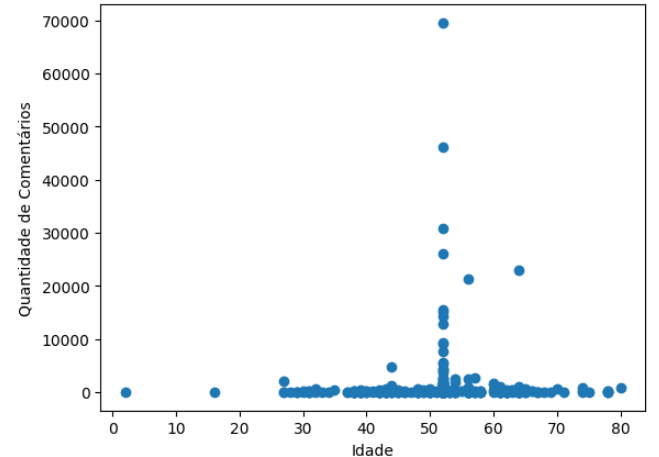
\includegraphics[scale=0.8]{images/colab_comments_by_age.png}
\end{figure}

Ao isolar as três cidades utilizadas como amostra nesse projeto, podem ser observados comportamentos distintos em cada uma. Nesse caso, Mesquita e Santo André apresentam comportamentos bastante semelhantes, com maior concentração dos usuários na faixa de 1-10 comentários. As três cidades possuem proporções similares nas faixas acima de 10 comentários.

\subsection*{Usuários com mais comentários}

Ao analisar os usuários com maior número de comentários, foram destacados os 1.000 usuários que mais comentam. A faixa etária desses usuários varia entre 16 e 84 anos, com representantes de 51 cidades distintas. As cidades com maior número de representantes são Niterói, Juiz de Fora e Santo André. De maneira geral, há predominância de homens (74\%), brancos (27\%), com ensino superior completo e uma mediana de idade de 45 anos.

\begin{figure}[!htb]
	\caption{Distribuição de Usuários por Quantidade de Comentários (por Cidade)}
	\label{fig:colab_comments_by_city}
	\centering
	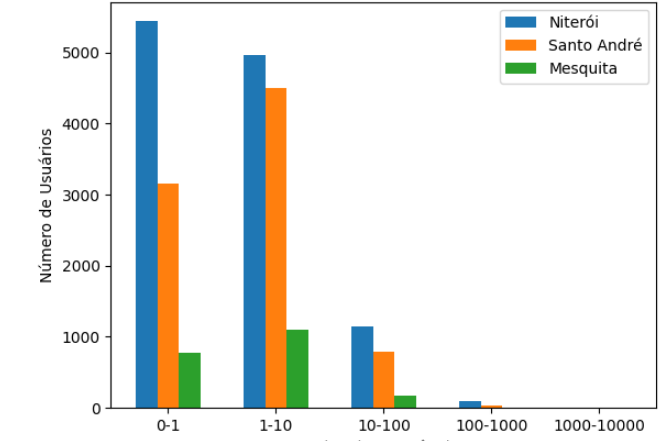
\includegraphics[scale=0.8]{images/colab_comments_by_city.png}
\end{figure}

\subsection*{Niterói, Mesquita e Santo André}

Para realizar análises mais aprofundadas, tanto de correlações quanto de análises de rede, foram selecionados os dados das três cidades com maior número de interações no Colab: Niterói, Santo André e Mesquita.

\subsection*{Correlação}

Com o objetivo de traçar um perfil dos usuários mais ativos na plataforma, buscou-se identificar alguma correlação entre a quantidade de atividades realizadas pelos cidadãos e suas principais características cadastrais (quando disponíveis). 

\begin{figure}[!htb]
	\caption{Matriz de Correlação}
	\label{fig:colab_correlation_matrix}
	\centering
	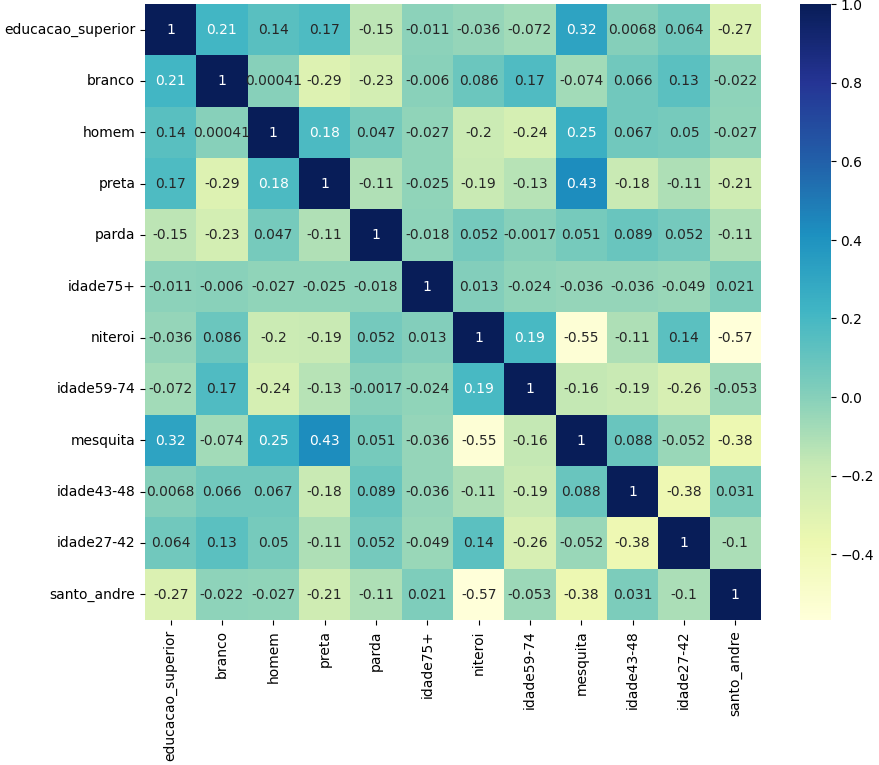
\includegraphics[scale=0.6]{images/colab_correlation_matrix.png}
\end{figure}

Para viabilizar a análise, algumas características foram transformadas em formato booleano (TRUE/FALSE). As características utilizadas foram:

\begin{itemize}
	\item Cidade do usuário, com destaque para Mesquita, Niterói e Santo André.
	\item Escolaridade, sendo considerado o nível "Superior +" que engloba ensino superior completo, mestrado e doutorado.
	\item Idade, com um recorte entre 10 e 90 anos e divisão em 5 faixas de tamanho igual: 10-26; 27-42; 43-58; 59-74; 75-90.
	\item Tipos de interações considerados para análise: comentários em publicações, curtidas em publicações, seguidores/seguindo e endosso ou rejeição de comentários .
	\item Cor/raça, incluindo as categorias branca, preta e parda.
	\item Gênero, considerando apenas homens.
	\item Número de interações acima da mediana do total de interações de cada usuário.
\end{itemize}

Com os dados disponíveis, não foi possível identificar características dos cidadãos que determinassem seu perfil de comportamento na plataforma. Portanto, não foram encontradas correlações relevantes para análise.

\begin{figure}[!htb]
	\caption{Matriz de Correlação}
	\label{fig:colab_correlation_bingo}
	\centering
	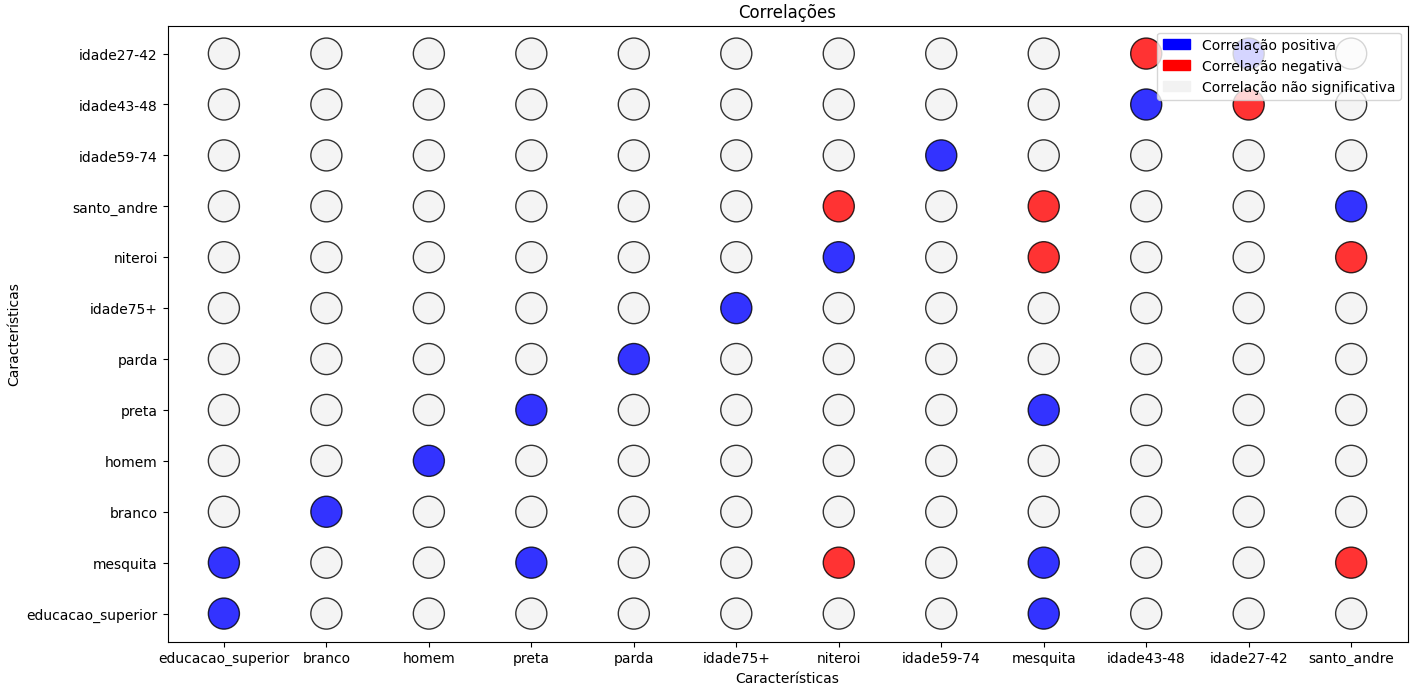
\includegraphics[scale=0.4]{images/colab_correlation_bingo.png}
\end{figure}

\subsection*{Regressão logística}

A fim de identificar características dos usuários que influenciam seu comportamento na plataforma, foi realizada uma regressão logística com base nas mesmas informações.

\begin{figure}[!htb]
	\caption{Regressão Logística}
	\label{fig:regression_chart}
	\centering
	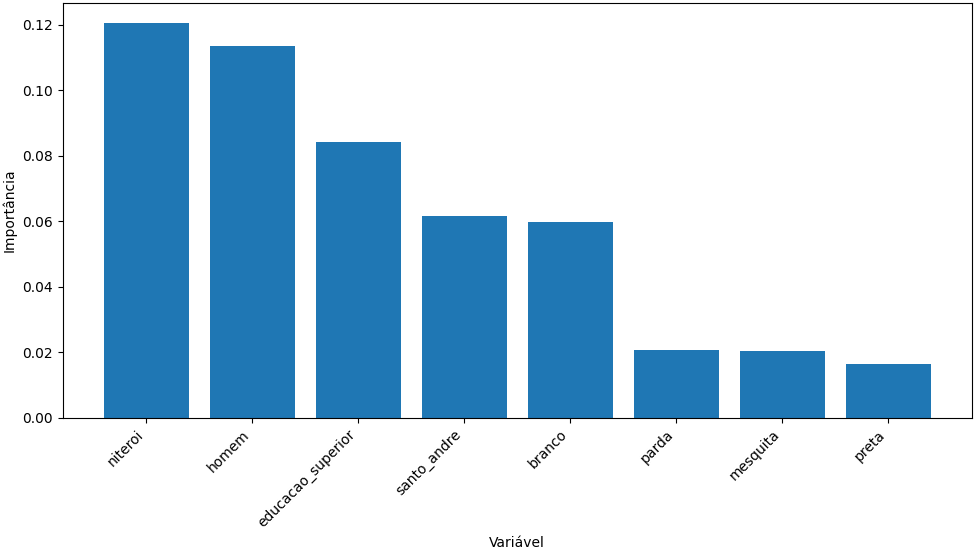
\includegraphics[scale=0.6]{images/regression_chart.png}
\end{figure}

A variável preditora utilizada foi o recorte no número de interações dos usuários: para aqueles que realizaram mais de 3 interações, ou seja, acima da mediana, foi atribuído o valor TRUE; para aqueles com interação menor que a mediana, FALSE.

A regressão logística apresentou uma AUC (área sob a curva ROC) baixa, indicando baixa precisão na previsibilidade das variáveis. No entanto, as variáveis preditoras mais relevantes foram:

\begin{itemize}
	\item Cidade de Niterói.
	\item Cor branca.
	\item Escolaridade compreendida entre ensino superior completo, mestrado e doutorado.
	\item Cor parda.
	\item Gênero masculino.
\end{itemize}

\begin{figure}[!htb]
	\caption{Regressão Logística - Curva ROC}
	\label{fig:regression_roc}
	\centering
	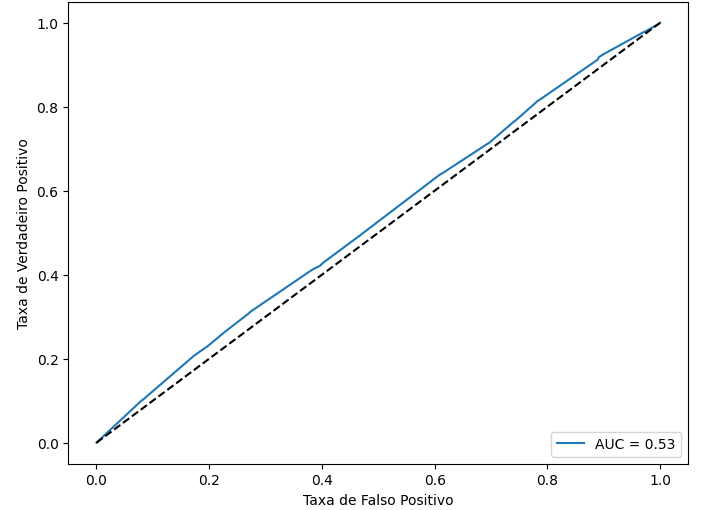
\includegraphics[scale=0.8]{images/regression_roc.png}
\end{figure}

\chapter{Compreendendo Câmaras de Eco e suas implicações}
\label{chapter:05_echochambers}
As mídias sociais revolucionaram a forma como as pessoas se comunicam e interagem umas com as outras. No entanto, o lado negativo dessa revolução é a crescente polarização e isolamento das pessoas em câmaras de eco. Uma câmara de eco pode ser definida como um sistema fechado em que as pessoas interagem apenas com aquelas que compartilham das mesmas crenças, valores e ideologias, enquanto ignoram ou suprimem ativamente pontos de vista opostos \cite[]{2015_Bakshy}. O termo "câmara de eco" tem origem no conceito de uma câmara de reverberação sonora, onde as ondas sonoras são refletidas entre as paredes, amplificando e distorcendo o som original.

Câmaras de eco podem ter sérias implicações para a sociedade, pois limitam a exposição a perspectivas diversas, levando ao reforço de crenças existentes e à exclusão de pontos de vista alternativos \cite[]{2001_Sunstein_BOOK}. Isso pode contribuir para a criação de uma divisão ideológica, que pode prejudicar o diálogo construtivo e o compromisso, resultando em uma sociedade polarizada e fragmentada. Além disso, câmaras de eco podem levar à disseminação de desinformação, propaganda e notícias falsas, uma vez que os indivíduos dentro desses sistemas fechados têm menos probabilidade de verificar a veracidade das informações que corroboram suas crenças existentes \cite[]{2016_Vicario}.

Compreender os mecanismos por trás da formação e manutenção das câmaras de eco é crucial para lidar com as consequências negativas associadas a esses fenômenos. A formação de câmaras de eco pode ser atribuída a diversos fatores, incluindo os algoritmos utilizados pelas plataformas de mídias sociais, os vieses cognitivos dos indivíduos e a influência de líderes de opinião \cite[]{2016_Flaxman}.

Em termos de fatores algorítmicos, as plataformas de mídias sociais utilizam algoritmos personalizados que visam fornecer aos usuários conteúdo alinhado com seus interesses, crenças e preferências. Isso significa que os indivíduos têm maior probabilidade de serem expostos a conteúdos que reforçam suas crenças e valores existentes, levando à formação de câmaras de eco \cite[]{2015_Bakshy}.

Vieses cognitivos, como viés de confirmação e exposição seletiva, também podem contribuir para a formação de câmaras de eco, pois os indivíduos tendem a buscar informações que confirmam suas crenças pré-existentes, enquanto ignoram ou rejeitam informações que as desafiam \cite[]{2006_Taber}. Além disso, líderes de opinião ou indivíduos com alta influência social podem desempenhar um papel na formação e manutenção das câmaras de eco, pois podem moldar as crenças e atitudes de seus seguidores \cite[]{2015_Bakshy}.

Câmaras de eco são um fenômeno preocupante nas mídias sociais, pois podem levar à polarização e fragmentação da sociedade, além da disseminação de desinformação e propaganda. Compreender os mecanismos por trás da formação e manutenção das câmaras de eco é crucial para mitigar suas consequências negativas.

\chapter{Explorando a História, Desenvolvimentos e Aplicações da Análise de Redes}
\label{chapter:06_networkanalysis}
Nesse capítulo, apresentamos os fundamentos da Análise de Redes Sociais. A análise de redes sociais (ARS) é uma abordagem que tem suas raízes na Sociometria e na Teoria dos Grafos, que são de viés matemático, para analisar relações sociais (Recuero, Bastos e Zago, 2015). A ideia central é que os indivíduos, ou atores sociais, estão inseridos em estruturas complexas de relações com outros atores, e essas estruturas têm um papel fundamental no comportamento e na visão de mundo desses indivíduos.

\subsection{Teoria dos Grafos}
A Teoria dos Grafos é um framework matemático que estuda as relações entre objetos e as conexões entre eles. As origens desta teoria estão no trabalho de Euler e na solução que ele propôs para o enigma das Pontes de Königsberg. A história relata que a cidade de Königsberg seria atravessada por sete pontes e que popularmente havia um desafio de desenhar um caminho por ela onde cada uma das pontes seria atravessada uma única vez. Euler teria demonstrado que tal desafio era impossível de ser resolvido utilizando um grafo, dando assim origem à teoria.

No livro "Introdução à análise de redes sociais online" de Raquel Recuero, a autora discute a importância da ARS e da Teoria dos Grafos para a compreensão das redes sociais online. Ela explica que a ARS permite a análise sistemática de grupos sociais a partir de sua estrutura, através de medidas específicas. A autora também destaca que a análise de redes sociais nasce de um ramo interdisciplinar de pesquisa, cujas bases podem ser encontradas nas mais variadas ciências, principalmente no início do século XX, particularmente, a partir da década de 1930.

Um conceito fundamental na Teoria dos Grafos é o de um "grafo", que é uma estrutura composta por "vértices" (ou "nós") e "arestas" que conectam esses vértices. Formalmente, um grafo $G$ é definido como um par ordenado $G := (V, E)$ compreendendo um conjunto $V$ de vértices ou nós juntamente com um conjunto $E$ de arestas ou arcos, que são pares de vértices (Bondy/Murty, 1976).

Os grafos podem ser categorizados como direcionados ou não direcionados. Em um grafo direcionado, as arestas têm uma direção associada, indicando uma relação unidirecional. Em contraste, em um grafo não direcionado, as arestas não têm direção, sugerindo uma relação bidirecional (West, 2001). Em termos de redes sociais, um exemplo de grafo direcionado seria o Twitter (onde um usuário pode seguir outro sem ser seguido de volta), enquanto um exemplo de grafo não direcionado seria o Facebook (onde a amizade é sempre mútua).

Outro conceito importante é o "grau" de um vértice, que é o número de arestas conectadas a ele. Em um grafo direcionado, distinguimos entre o "grau de entrada" (o número de arestas que entram no vértice) e o "grau de saída" (o número de arestas que saem do vértice). O grau de um vértice pode ser usado para medir sua importância ou influência dentro da rede (Newman, 2010).

Um "caminho" em um grafo é uma sequência de vértices na qual cada vértice é conectado ao próximo por uma aresta. O "comprimento" de um caminho é o número de arestas que ele contém. Este conceito é crucial para entender como a informação ou influência pode se propagar através da rede (Easley/Kleinberg, 2010).

A "conectividade" de um grafo é uma medida de quão integrada ou unida é a rede. Um grafo é dito "conectado" se houver um caminho entre cada par de vértices (West, 2001).

Um "subgrafo" é um grafo formado a partir de um conjunto de vértices e arestas de um grafo maior. Os subgrafos podem ser usados para estudar partes específicas de uma rede (West, 2001).

Recuero também enfatiza a diferença entre redes sociais e sites de rede social. Enquanto uma rede social está relacionada à percepção de um grupo social determinado pela sua estrutura (a “rede”), que é geralmente oculta, pois só está manifesta nas interações, as ferramentas sociais na internet são capazes de publicizar e influenciar essas estruturas sociais. Assim, o Facebook, por si só, não apresenta redes sociais. É o modo de apropriação que as pessoas fazem dele que é capaz de desvelar redes que existem ou que estão baseadas em estruturas sociais construídas por essas pessoas.

Portanto, a Teoria dos Grafos e a Análise de Redes Sociais são ferramentas essenciais para a compreensão das complexas redes de interações sociais que se formam tanto no mundo offline quanto online. Elas permitem uma visão mais profunda e sistemática das relações sociais, contribuindo para uma melhor compreensão dos fenômenos sociais.

\subsection{Grafos Sociais}

Um dos primeiros desenvolvimentos na análise de redes foi o trabalho do sociólogo Georg Simmel no início do século XX. Simmel aplicou os princípios da teoria dos grafos às relações sociais, argumentando que as estruturas sociais surgem a partir dos padrões de interação entre os indivíduos \cite[]{2021_Hollstein}. Desde então, a análise de redes tem sido aplicada em uma ampla gama de campos, incluindo ciência da computação, física, biologia e ciências sociais, entre outros.

Simmel foi pioneiro em determinar a interação social como o bloco de construção básico da sociologia, indo além de seus contemporâneos, como Spencer. Ele argumentou que para entender o comportamento social, devemos estudar os padrões de interação, oferecendo insights penetrantes sobre a dinâmica das relações sociais. Embora Simmel nunca tenha usado o termo "rede social", muitos analistas de rede o consideram um precursor importante da abordagem de rede social.

Além disso, a análise de redes tem sido usada para entender a estrutura e a dinâmica de "redes escuras", como redes de criminosos ou terroristas. A análise de redes também tem sido aplicada para entender a estrutura e a dinâmica das organizações e como a estrutura da rede pode afetar a eficácia e a eficiência organizacional.

No entanto, apesar do rápido crescimento da análise de redes nas últimas duas décadas, as críticas à abordagem também aumentaram. Alguns críticos argumentam que a análise de redes pode ser excessivamente determinística, ignorando a agência individual e a complexidade das relações sociais (Scott, 1991). Além disso, a análise de redes pode ser desafiadora devido à dificuldade de coletar dados completos e precisos sobre redes sociais.

A análise de redes sociais tem sido criticada por sua falta de consideração pelos aspectos qualitativos das redes sociais e por sua tendência a simplificar as complexidades das interações sociais (Haythornthwaite, 2013). Além disso, a análise de redes sociais é frequentemente criticada por sua falta de consideração pelos aspectos contextuais das redes sociais e por sua ênfase excessiva em padrões estruturais (What is Social Network Analysis, n.d.).

Essas críticas destacam a necessidade de abordagens mais holísticas e integradas para a análise de redes sociais, que levem em consideração tanto os aspectos quantitativos quanto qualitativos das redes sociais, bem como os contextos sociais e culturais em que essas redes estão inseridas.

\subsection{Centralidade e Comunidades}

Um método comum usado na análise de redes é a análise de centralidade, que mede a importância dos nós na rede com base em sua posição e conexões dentro da rede \cite[]{1978_Freeman}. Medidas de centralidade podem ajudar a identificar atores-chave na rede, ou nós que desempenham papéis importantes como porteiros, conectores ou intermediários entre diferentes partes da rede.

Outro método importante na análise de redes é a detecção de comunidades, que identifica grupos de nós que estão mais densamente conectados entre si do que com o restante da rede \cite[]{2004_Newman}. A detecção de comunidades pode ajudar a identificar grupos de indivíduos com atributos ou comportamentos semelhantes, ou grupos que são mais suscetíveis à propagação de informações ou influências.

\subsection{Aplicações da Análise de Redes}

A análise de redes tem sido aplicada em uma ampla gama de campos, além das redes sociais, com aplicações que vão desde redes de transporte até a neurociência. No campo do transporte, a análise de redes tem sido usada para estudar o fluxo de tráfego nas estradas e identificar áreas de gargalo que podem ser melhoradas para aumentar a eficiência do tráfego \cite[]{2012_Levinson}. Por exemplo, \citeonline{2010_Bierlaire} aplicaram a análise de redes para otimizar o sistema de transporte público, reduzindo o tempo de viagem e melhorando a eficiência do serviço. No campo acadêmico, a análise de redes tem sido aplicada para estudar as redes de coautoria na publicação acadêmica. \citeonline{2001_Newman} utilizou a análise de redes para estudar os padrões de colaboração entre autores e a emergência de comunidades de pesquisa. No campo organizacional, a análise de redes tem sido usada para compreender a estrutura de padrões de comunicação formais e informais em organizações. \citeonline{2004_Cross_BOOK} utilizaram a análise de redes para entender como os indivíduos influenciam os processos de tomada de decisão e a emergência de estruturas de poder dentro das organizações. Na biologia, a análise de redes tem sido usada para estudar redes de interação de proteínas, redes regulatórias de genes e redes metabólicas \citeonline{2004_Barabasi} utilizaram a análise de redes para entender como as proteínas interagem entre si em uma célula, fornecendo insights sobre como as doenças afetam essas interações.
\begin{figure}[!htb]
    \caption{Imagem ilustrativa de uma rede de interação de proteínas}
    \label{fig:network_proteins}
    \centering
    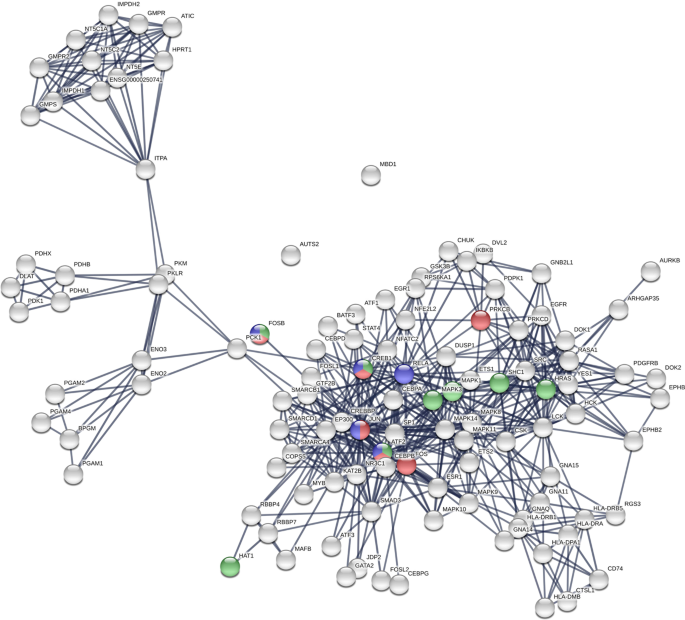
\includegraphics[scale=0.5]{network_proteins.png}
    \fdireta{2004_Barabasi}
\end{figure}
A análise de redes também tem sido usada em neurociência para estudar redes cerebrais. Por exemplo, pesquisadores têm utilizado a análise de redes para entender como diferentes regiões do cérebro interagem entre si, o que pode ajudar a entender doenças como a esquizofrenia e o Alzheimer \cite[]{2009_Bullmore}.
\begin{figure}[!htb]
    \caption{Imagem ilustrativa de uma rede de interação de proteínas}
    \label{fig:network_brain}
    \centering
    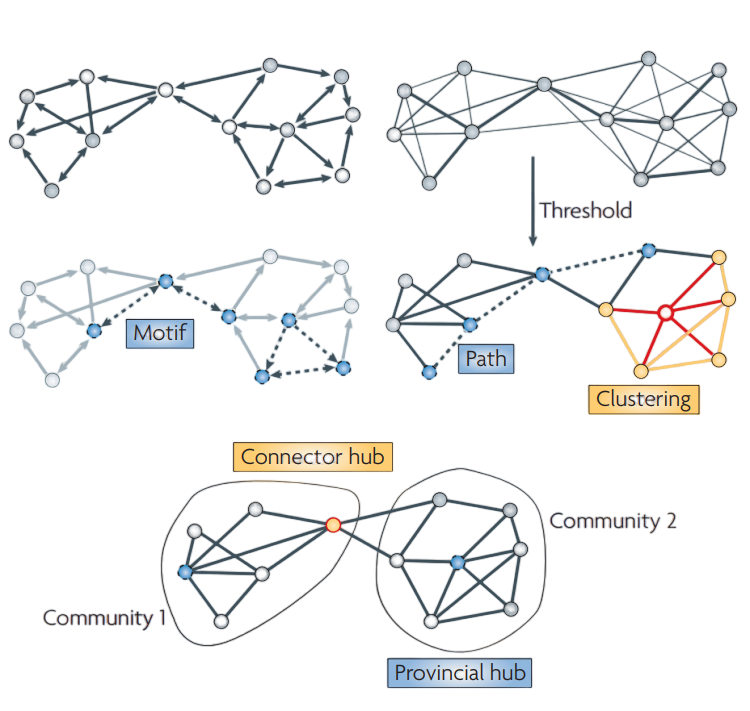
\includegraphics[scale=0.25]{network_brain.png}
    \fdireta{2009_Bullmore}
\end{figure}

\subsection{Epidemiologia e Redes Complexas}
Na epidemiologia, a análise de redes tem se mostrado uma abordagem fundamental para estudar a transmissão de doenças infecciosas e entender a estrutura dos contatos entre indivíduos infectados. Dentre as diversas contribuições nesse campo, destaca-se o livro "Mathematics of Epidemics on Networks" \cite[]{2017_Kiss_BOOK}, que explora a aplicação do modelo SIR (Susceptível-Infectado-Recuperado) em redes complexas, em que os nós representam indivíduos e as arestas representam as interações entre eles. O livro desvenda como a estrutura da rede pode influenciar a propagação de doenças, investigando questões como o papel dos nós centrais na disseminação das enfermidades, a eficácia de diferentes estratégias de controle e intervenções, bem como o impacto de características topológicas específicas na dinâmica das epidemias. Uma das contribuições centrais do livro é a introdução do conceito de estrutura de redes em formato de gravata borboleta, a qual permite uma análise mais profunda e abrangente das redes complexas. 
Essa estrutura é composta por três principais componentes: a Área Central (SCC), a Seção de Entrada (IN) e a Seção de Saída (OUT). Matematicamente, podemos representar esses componentes de acordo com o seguinte modelo:

\begin{equation}
\text{{SCC}} = { v \in V : \forall u,w \in \text{{SCC}}, \text{{existe um caminho direto de }} u \text{{ para }} w }
\end{equation}

\begin{equation}
\text{{IN}} = { v \in V : \exists u \in \text{{SCC}}, \text{{ tal que }} (u,v) \in E \text{{ e não existe um caminho direto de }} v \text{{ para }} u }
\end{equation}

\begin{equation}
\text{{OUT}} = { v \in V : \exists u \in \text{{SCC}}, \text{{ tal que }} (v,u) \in E \text{{ e não existe um caminho direto de }} u \text{{ para }} v }
\end{equation}

Onde $V$\simbolo{V}{Representa um conjunto de nós em um grafo} representa o conjunto de nós e $E$\simbolo{E}{Representa um conjunto de arestas em um grafo} o conjunto de arestas da rede. A Área Central {SCC} consiste em nós altamente conectados, em que há um caminho direto de um nó para qualquer outro nó da área central. A Seção de Entrada {IN} é composta por nós que possuem conexões direcionadas para a área central, mas não têm caminhos de retorno diretos para os nós da Seção de Saída {OUT} ou da área central. Analogamente, a Seção de Saída {OUT} inclui nós que têm conexões direcionadas da área central, mas não possuem caminhos de retorno diretos para os nós da Seção de Entrada {IN} ou da área central.

Essa estrutura de redes em formato de gravata borboleta tem o potencial de ser aplicada para interpretar grafos direcionados em redes sociais. Ao analisar uma rede social, podemos identificar a Área Central {SCC} como os indivíduos ou grupos altamente conectados que desempenham um papel central na propagação de informações ou influência na rede. A Seção de Entrada {IN} representa os nós que interagem com a Área Central, mas não possuem conexões diretas entre si. Esses nós podem desempenhar um papel crucial ao receber informações da Área Central e disseminá-las para outros nós da rede. Da mesma forma, a Seção de Saída {OUT} inclui os nós que têm conexões direcionadas para a Área Central, mas não estão diretamente conectados uns aos outros. Esses nós podem ser responsáveis por disseminar informações ou influência da Área Central para outras partes da rede.

A propagação de fake news em redes sociais pode ser comparada à disseminação de doenças infecciosas, em que a informação falsa se espalha de maneira semelhante a um contágio. A estrutura de redes em formato de gravata borboleta, descrita no livro, pode ajudar a identificar os nós centrais e influentes que desempenham um papel importante na disseminação de informações falsas. Além disso, a análise da dinâmica da propagação de fake news pode se beneficiar das técnicas e modelos matemáticos discutidos no livro para compreender a rapidez e o alcance dessa disseminação.

Uma outra contribuição importante é na epidemiologia não Markoviana. Os modelos estocásticos de epidemias não markovianas (Stochastic non-Markovian epidemics) são uma extensão dos modelos clássicos de epidemias, que consideram a dependência temporal e complexa das interações entre os eventos em um processo epidêmico. Esses modelos reconhecem que a probabilidade de transição entre estados pode depender do histórico completo de estados anteriores, levando em conta fatores como a história de exposição, imunidade adquirida e comportamentos individuais. Matematicamente, podemos representar um modelo estocástico de epidemia não markoviana como:

\begin{equation}
P(S(t+\Delta t), I(t+\Delta t), R(t+\Delta t)|S(t), I(t), R(t), \mathcal{H}(t))
\end{equation}

onde $S(t)$, $I(t)$ e $R(t)$ representam o número de indivíduos suscetíveis, infectados e recuperados no tempo $t$, respectivamente, e $\mathcal{H}(t)$ denota o histórico completo dos eventos até o tempo $t$.

A aplicação dos modelos estocásticos de epidemias não markovianas na análise de redes sociais pode fornecer insights importantes para entender fenômenos como polarização e câmaras de eco. Ao considerar a dependência temporal nas interações sociais, esses modelos podem capturar como a exposição a determinadas opiniões ou informações no passado influencia a propensão de um indivíduo em adotar ou compartilhar essas opiniões no futuro. Essa dependência temporal pode ser representada por meio de uma função de probabilidade condicional:

\begin{equation}
P(I(t+\Delta t)|I(t), \mathcal{H}(t))
\end{equation}

Essa abordagem permite investigar como a formação e a propagação de polarização e câmaras de eco ocorrem ao longo do tempo em uma rede social. Por exemplo, pode-se analisar como a exposição a opiniões semelhantes influencia a adesão a um grupo específico e a formação de câmaras de eco, onde informações são amplificadas e reforçadas dentro de determinados grupos, resultando em uma maior polarização entre eles. Além disso, a aplicação desses modelos permite explorar o papel dos nós centrais na disseminação de polarização, bem como o impacto de intervenções e estratégias de controle na quebra das câmaras de eco e na redução da polarização.

Dessa forma, a utilização de modelos estocásticos de epidemias não markovianas na análise de redes sociais oferece uma abordagem poderosa para investigar e compreender os mecanismos subjacentes à formação de polarização e câmaras de eco. A inclusão da dependência temporal e das interações complexas entre os indivíduos permite uma representação mais realista dos processos sociais em redes complexas, proporcionando insights valiosos para o desenvolvimento de estratégias de mitigação e intervenções eficazes no combate à polarização e à formação de câmaras de eco em redes sociais.

A integração de eventos estocásticos, no contexto das redes sociais, pode ser relacionada aos momentos de grande tráfego ou atividade intensa nessas plataformas. Esses eventos podem ser caracterizados por um aumento significativo no número de interações, compartilhamentos, curtidas e comentários em determinados conteúdos. Matematicamente, podemos representar esses eventos estocásticos como:

\begin{equation}
P(S(t+\Delta t), I(t+\Delta t), R(t+\Delta t)|S(t), I(t), R(t), \mathcal{H}(t), \mathcal{T}(t))
\end{equation}

onde $\mathcal{T}(t)$ denota o histórico completo dos eventos de tráfego e atividade na rede social até o tempo $t$.

A introdução de hashtags como dados de entrada nessa análise pode ser feita considerando-as como fatores de disseminação de informações análogos ao contágio na epidemiologia clássica. A presença e popularidade de uma hashtag específica podem influenciar a propagação de informações relacionadas a um determinado tópico na rede social. Isso pode ser representado matematicamente pela função de probabilidade condicional:

\begin{equation}
P(I(t+\Delta t)|I(t), \mathcal{H}(t), \mathcal{T}(t), \mathcal{C}(t))
\end{equation}

onde $\mathcal{C}(t)$ representa o conjunto de hashtags relevantes e populares até o tempo $t$.

A inclusão das hashtags nessa análise permite uma compreensão mais abrangente e precisa da disseminação de informações nas redes sociais. Elas atuam como marcadores temáticos e podem desempenhar um papel importante na formação de comunidades online, na viralização de conteúdos específicos e na amplificação de certas mensagens. As hashtags funcionam como vetores de contágio, direcionando a atenção dos usuários para tópicos específicos e influenciando a propagação de informações relacionadas.

Ao incorporar as hashtags como fator de disseminação de informação na análise estocástica de redes sociais, é possível investigar como sua presença e popularidade influenciam a adesão dos usuários a determinados tópicos, a propagação de informações e a formação de comunidades temáticas. A análise da dependência temporal e da interação complexa entre as hashtags e o histórico de eventos na rede social pode fornecer insights valiosos sobre a dinâmica da disseminação de informações e ajudar a identificar padrões de comportamento e tendências emergentes.

Em resumo, a integração de eventos estocásticos no contexto das redes sociais, juntamente com a consideração das hashtags como fator de disseminação de informação análoga ao contágio na epidemiologia clássica, permite uma análise mais abrangente e precisa da propagação de informações e da formação de comunidades temáticas. Essa abordagem contribui para a compreensão dos processos sociais em redes complexas, fornecendo insights valiosos para a identificação de tendências, a criação de estratégias de engajamento e o desenvolvimento de intervenções eficazes na disseminação de informações em redes sociais.

\citeonline{2005_Christley} utilizaram a análise de redes para entender como a gripe se espalha em uma população, o que pode ajudar a desenvolver estratégias de prevenção mais eficazes.
\begin{figure}[!htb]
    \caption{Ilustração esquemática de uma topologia em formato de gravata borboleta}
    \label{fig:network_bowtie}
    \centering
    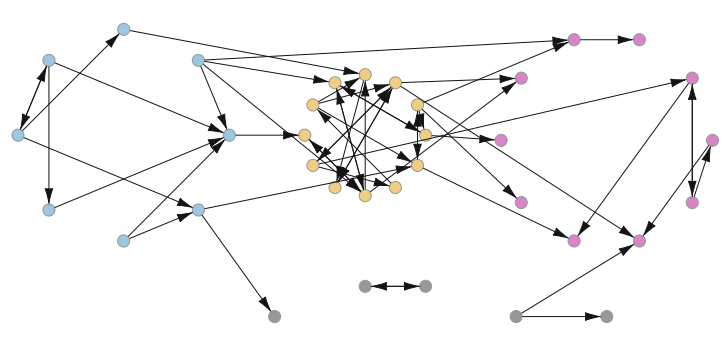
\includegraphics[width=\textwidth]{network_bowtie.png}
    \fdireta{2017_Kiss_BOOK}
\end{figure}

\subsection{Análise de Redes Sociais Online}

Outra importante aplicação da análise de redes está no estudo de comunidades online e mídias sociais. O crescimento exponencial de plataformas online e redes sociais tem fornecido aos pesquisadores vastas quantidades de dados para analisar a dinâmica dessas comunidades. Por exemplo, um estudo de utilizou a análise de redes para investigar a estrutura e dinâmica das comunidades de discussão online no Reddit. O estudo constatou que as comunidades exibiam uma estrutura hierárquica com subcomunidades distintas que se formavam em torno de tópicos específicos. Outro estudo de \citeonline{2011_Quercia_IP} utilizou a análise de redes para estudar a influência de relacionamentos sociais na propagação de informações no Twitter. O estudo constatou que a estrutura da rede social influenciava a propagação de informações, sendo que clusters densamente conectados tinham maior probabilidade de promover a difusão de informações do que clusters esparsamente conectados.

Em conclusão, a análise de redes é uma ferramenta poderosa para analisar sistemas complexos e compreender as relações entre seus componentes. Ela tem suas origens na teoria dos grafos e se desenvolveu em um campo multidisciplinar com aplicações em várias áreas, como redes sociais, comunidades online, epidemiologia, ecologia e transporte. A aplicação da análise de redes em redes sociais tem levado a insights importantes sobre a estrutura e dinâmica dessas redes e tem ajudado os pesquisadores a compreender os mecanismos de influência social e a propagação de informações. O uso da análise de redes em outros campos também tem levado a descobertas importantes e tem o potencial de aprimorar nossa compreensão dos sistemas que moldam nosso mundo.

\chapter{Análise de Redes Sociais no Brasil}
\label{chapter:07_networkbr}
Análise de Redes Sociais (ARS) é uma ferramenta poderosa para analisar a estrutura e dinâmica de redes sociais. No Brasil, ela tem sido amplamente utilizada nas últimas décadas para estudar diversos fenômenos, como comportamento organizacional, redes políticas, crime e redes de inovação. Este artigo apresenta um resumo breve da ARS no Brasil, destacando suas principais contribuições teóricas e metodológicas, bem como os desafios que enfrenta.

Um dos temas-chave da ARS no Brasil tem sido o estudo do capital social e seu impacto nos resultados sociais e econômicos. Pesquisas nessa área têm mostrado que as redes sociais podem facilitar a troca de recursos, conhecimentos e oportunidades, e que elas podem desempenhar um papel importante na promoção da mobilidade social e no desenvolvimento econômico (Costa/Granja, 2019). No entanto, a pesquisa em ARS no Brasil também tem mostrado que o capital social pode ser excludente, reforçando relações de poder existentes e perpetuando a desigualdade (Brasileiro/Gomes, 2015).

Outra área de pesquisa que tem sido proeminente na ARS no Brasil é o estudo das redes interorganizacionais. Estudos nessa área têm mostrado como as redes de empresas podem afetar a inovação, a difusão de conhecimento e a competitividade, bem como como elas podem moldar a governança de setores e regiões (Pereira/Vieira, 2018). No entanto, a pesquisa em ARS no Brasil também revelou que as redes interorganizacionais podem ser altamente fragmentadas e desconectadas, limitando o potencial para ação coletiva e cooperação (Brasileiro/Gomes, 2015).

Redes políticas também têm sido um foco importante da ARS no Brasil, especialmente no contexto da corrupção e do clientelismo. Pesquisas nessa área têm mostrado como as redes de políticos, funcionários públicos e grupos de interesse podem moldar os resultados políticos e perpetuar comportamentos de busca de benefícios pessoais (Codato, 2015). A pesquisa em ARS no Brasil também tem revelado os desafios de estudar redes políticas, incluindo a disponibilidade limitada de dados e a sensibilidade do tema.

Crime e tráfico de drogas têm sido outra área importante de pesquisa em ARS no Brasil. Estudos nessa área têm utilizado a ARS para analisar a estrutura e dinâmica de redes criminosas, identificando atores-chave e seus papéis na produção e distribuição de bens ilícitos (Martins/Lima, 2018). No entanto, a pesquisa em ARS no Brasil também tem revelado as dificuldades de estudar redes criminosas, incluindo os riscos e preocupações éticas de coletar dados sobre atividades ilegais.

Nos últimos anos, a pesquisa em ARS no Brasil também tem explorado novas aplicações e abordagens metodológicas. Por exemplo, alguns estudos têm utilizado a ARS para analisar redes sociais e comunidades online, investigando como elas moldam a opinião pública e a mobilização política (Gonçalves et al., 2020). Outros têm combinado a ARS com métodos qualitativos, como entrevistas e etnografia, para obter uma compreensão mais profunda das dinâmicas sociais e culturais das redes (Brandão et al., 2019).

Apesar do potencial da ARS no Brasil, essa abordagem também enfrenta vários desafios. Um dos principais desafios é a disponibilidade limitada e a qualidade dos dados, especialmente no contexto de temas sensíveis, como política e crime. Pesquisadores também apontaram a necessidade de desenvolver novos métodos para analisar redes dinâmicas e heterogêneas, bem como a importância de considerar o contexto cultural e histórico das redes (Brasileiro/Gomes, 2015; Pereira/Vieira, 2018).

Em conclusão, a ARS tem sido uma ferramenta valiosa para compreender redes sociais no Brasil, contribuindo para nosso conhecimento sobre capital social, redes interorganizacionais, redes políticas e crime. No entanto, essa abordagem também enfrenta desafios, como a disponibilidade de dados e limitações metodológicas. Futuras pesquisas em ARS no Brasil devem buscar enfrentar esses desafios ao mesmo tempo em que exploram novas aplicações e perspectivas teóricas.

\chapter{Análise Exploratória de Redes}
\label{chapter:08_exploratory}
Nesta seção, exploramos o uso da análise de redes para analisar o conjunto de dados Colab.re. O conjunto de dados consiste em uma lista de arestas, onde os nós são usuários e as arestas representam as conexões ou seguidores desses usuários. O objetivo deste estudo é identificar câmaras de eco na rede Colab.re e obter insights sobre a estrutura dessas comunidades.

Para alcançar isso, utilizamos várias técnicas de análise de redes, como agrupamento de Louvain, agrupamento espectral e autovetores. O agrupamento de Louvain é um algoritmo de detecção de comunidades que otimiza a modularidade, uma medida da densidade de conexões dentro das comunidades em comparação com as conexões entre comunidades. O agrupamento espectral é uma técnica que utiliza os autovalores e autovetores do Laplaciano do grafo para particionar o grafo em comunidades. Por outro lado, os autovetores são usados para identificar os nós centrais na rede, também conhecidos como "centralidade de autovetor".

Este estudo baseia-se em pesquisas anteriores que utilizaram a análise de redes para estudar redes sociais, como o Twitter e o Facebook, a fim de obter insights sobre a estrutura dessas comunidades. Por exemplo, \citeonline{2006_Newman} utilizaram o agrupamento espectral para identificar comunidades em uma rede de blogs políticos e mostraram que essas comunidades eram altamente polarizadas.

\section{Introdução ao Gephi}

A análise exploratória de redes sociais (ESNA) é um passo fundamental para compreender as estruturas complexas e dinâmicas das redes sociais. O primeiro passo na ESNA é visualizar os dados da rede, e o Gephi é uma das ferramentas mais populares e poderosas usadas nessa etapa. O Gephi é um software de análise e visualização de redes de código aberto que permite aos pesquisadores criar e manipular grafos, executar vários algoritmos de análise de rede e gerar representações visuais das estruturas de rede. O Gephi tem sido amplamente utilizado na análise de redes sociais (SNA) para analisar a estrutura e dinâmica dos relacionamentos sociais.

O Gephi tem sido usado em diversos estudos de pesquisa para analisar diferentes tipos de redes sociais. Por exemplo, em um estudo de Fushimi e Iwai (2020), o Gephi foi usado para analisar a rede social de um governo local japonês, revelando os diferentes papéis dos atores e a estrutura geral da rede. Da mesma forma, em um estudo de Kim et al. (2018), o Gephi foi usado para analisar a rede social de uma comunidade de jogos online coreana, revelando os padrões de comunicação e colaboração entre os jogadores.

O Gephi possui muitos dos modelos e algoritmos mais comuns de SNA, como centralidade de grau, centralidade de intermediação e coeficiente de agrupamento. Essas medidas permitem que os pesquisadores examinem a importância de nós ou atores individuais dentro de uma rede, bem como a estrutura geral da rede. O software também inclui uma variedade de algoritmos de layout que permitem aos pesquisadores visualizar as estruturas de rede de diferentes maneiras, como o layout ForceAtlas2, que simula forças físicas entre os nós para criar uma representação visual clara da rede.

O Gephi também pode ser usado para analisar a dinâmica temporal das redes sociais. Por exemplo, em um estudo de Zhang et al. (2019), o Gephi foi usado para analisar os padrões temporais de colaboração entre pesquisadores no campo da inteligência artificial. Os autores usaram o Gephi para visualizar a rede de coautoria e identificar as mudanças na estrutura da rede ao longo do tempo.

Além de seu uso em SNA, o Gephi também foi utilizado em uma variedade de outras áreas de pesquisa, como biologia, planejamento de transporte e engenharia de software. Por exemplo, em um estudo de Zhang et al. (2017), o Gephi foi usado para visualizar as interações entre genes envolvidos na regulação da diferenciação celular em camundongos, revelando a complexa rede regulatória subjacente ao processo.

Outra característica útil do Gephi é sua capacidade de lidar com conjuntos de dados grandes e complexos. O Gephi pode lidar com redes com milhões de nós e arestas, tornando-se uma ferramenta valiosa para analisar redes sociais em larga escala. Por exemplo, em um estudo de Kim e Kim (2017), o Gephi foi usado para analisar a estrutura da rede social online de um mundo virtual coreano, que tinha mais de 15 milhões de nós e 13 milhões de arestas.

Particularmente para este estudo, uma área em que o Gephi tem sido útil é na detecção de câmaras de eco em redes sociais. Por exemplo, em um estudo de \citeonline{2021_Conover}, o Gephi foi usado para analisar as conversas no Twitter em torno das eleições legislativas dos Estados Unidos em 2010, revelando a existência de comunidades ideologicamente segregadas.

Para detectar câmaras de eco usando o Gephi, os pesquisadores primeiro precisam coletar dados sobre a rede social de interesse. Isso pode ser feito usando uma variedade de métodos, como web scraping, chamadas de API ou pesquisas. Uma vez que os dados são coletados, eles podem ser importados para o Gephi e visualizados usando as ferramentas de visualização de rede do software. Os pesquisadores podem então usar vários algoritmos de SNA para identificar os nós mais centrais dentro da rede, bem como as diferentes comunidades ou subgrupos dentro da rede.

\section{Pré-processamento do conjunto de dados Colab.re}

Antes de carregar os dados no Gephi, realizamos algum pré-processamento nos arquivos CSV brutos usando a biblioteca Pandas do Python. O CSV original era uma lista de arestas em que a coluna "source" representava um usuário e a coluna "target" representava uma conexão com outro usuário. O arquivo CSV também tinha colunas para registrar quando essas relações foram criadas, atualizadas e excluídas, o que pode ser usado para adicionar dinâmica temporal à visualização. No entanto, os carimbos de data e hora originais estavam no formato brasileiro e precisaram ser convertidos para o formato ISO 8601, que é o padrão do Gephi.

Outra etapa foi separar a tabela de arestas dos dados dos nós, dedicando um arquivo para as relações dos usuários expressas por meio das colunas "source" e "target", e outro arquivo para os dados dos nós dos usuários. Esses arquivos são edges.csv e nodes.csv, respectivamente. Neste momento, o arquivo de nós contém apenas dados temporais, mas mais adiante no experimento, pretendemos incorporar também dados de localização, por isso decidimos dividir os arquivos. Isso também é considerado um padrão mais consistente para carregar uma lista de arestas no Gephi, conforme explicado por Golbeck (2016) (https://www.youtube.com/watch?v=HJ4Hcq3YX4k).

Também removemos nós duplicados. No contexto dos dados brutos, a coluna 'deleted\_at' representa quando um usuário foi deixado de seguir por outro usuário. Essa métrica nos fornece uma visão mais ampla do modelo de comunidade, mas, por simplicidade, optamos por removê-la deste primeiro experimento no Gephi. Retomaremos o estudo sobre a ação de deixar de seguir usuários posteriormente.

Para aproveitar o poder computacional, usamos o Google Colaboratory para realizar o pré-processamento dos dados. O script abaixo adapta as colunas de carimbos de data e hora e remove as linhas duplicadas.

\section{Carregando o conjunto de dados Colab.re no Gephi}
Após baixar o arquivo pré-processado, criamos um novo Workspace no Gephi e carregamos os arquivos de dados separadamente, começando pelo edges.csv, conforme explicado por Golbeck (2016).

O arquivo nodes.csv é então carregado e o Gephi detecta automaticamente os carimbos de data e hora.

Após importar ambos os arquivos, a tabela de dados do Gephi exibe os nós, as arestas e os carimbos de data e hora.

A importação detectou 33818 nós e 66877 arestas.

No entanto, devido ao alto número de conexões, a visualização do gráfico do Gephi exibe apenas um quadrado preto. Para corrigir isso e obter informações iniciais do conjunto de dados, precisamos escolher um Layout apropriado usando a guia de layout do Gephi.

\section{Compreendendo os Layouts do Gephi}

Os layouts são um aspecto essencial da funcionalidade do Gephi, pois eles fornecem uma representação gráfica da estrutura da rede. O Gephi oferece vários presets de layout para gerar visualizações dos dados da rede em diversas formas. Cada preset utiliza um conjunto único de algoritmos para posicionar os nós e arestas da rede de maneira visualmente atraente. Nesta seção, examinaremos alguns dos layouts mais comuns do Gephi, seus casos de uso e sugeriremos o melhor layout para uma rede com tantas conexões.

Um dos layouts mais utilizados no Gephi é o layout Force Atlas. O layout Force Atlas é um layout baseado em forças que simula a física de um sistema massa-mola para organizar os nós da rede. Esse layout é particularmente útil para visualizar redes sociais, pois pode destacar aglomerados e comunidades de nós. O layout Force Atlas é especialmente adequado para redes de tamanho pequeno a médio, pois pode se tornar computacionalmente caro para redes maiores.

O layout Fruchterman-Reingold é outro layout popular no Gephi. Também é um layout baseado em forças que equilibra as forças de atração e repulsão entre os nós. Esse layout é particularmente útil para visualizar redes de tamanho pequeno a médio e pode ser usado para destacar aglomerados e comunidades de nós.

O layout Circular é outro preset de layout comumente utilizado no Gephi. Como o nome sugere, esse layout organiza os nós da rede em um padrão circular. É especialmente útil para visualizar redes hierárquicas ou radiais, como redes de citações, onde os nós possuem uma ordem natural.

O layout Yifan Hu é um algoritmo baseado em forças desenvolvido por Yifan Hu em 2005. O algoritmo utiliza uma abordagem multinível para otimizar o layout dos nós em uma rede, minimizando uma função de energia que equilibra as forças de repulsão e atração entre os nós. Em cada nível, o algoritmo constrói uma representação mais grosseira da rede e a utiliza para guiar o layout da rede em níveis mais finos. Essa abordagem permite que o algoritmo lide com redes grandes e complexas, reduzindo a complexidade computacional do processo de layout. O layout Yifan Hu foi integrado em várias ferramentas de visualização de redes, incluindo o Gephi, como uma opção de layout padrão. A eficácia do layout foi demonstrada em diversos estudos, incluindo um estudo realizado por Lin (2019), que utilizaram o layout para visualizar a rede de coautoria de uma disciplina científica. Os resultados mostraram que o layout Yifan Hu foi capaz de visualizar efetivamente a estrutura da comunidade e destacar autores e publicações importantes dentro da rede.

Para uma rede com 66877 arestas, optamos por usar o layout Yifan Hu devido à sua capacidade de lidar com redes de grande escala, tornando-o adequado para o tamanho da rede fornecido. Além disso, o layout Yifan Hu é baseado em forças e pode otimizar o layout dos nós para fornecer uma representação visualmente agradável da rede. Posteriormente no experimento, pretendemos utilizar outros modelos de layout para obter diferentes insights do modelo de dados.

\section{Visualizações do Gephi da Rede Colab.re}

O layout Yifan Hu foi aplicado ao conjunto de dados do Colab.re, resultando nesta imagem que apresenta dois clusters bem populados, uma quantidade considerável de nós de usuário e um grande número de nós isolados.

O Yifan Hu nos proporciona um bom ponto de partida e algumas ideias iniciais. No entanto, para obter mais informações sobre o conjunto de dados, precisamos executar algumas estatísticas no Gephi e atualizar a aparência da visualização com os resultados das estatísticas. Vamos começar introduzindo as várias estatísticas do Gephi e avaliar como nossa análise de câmara de ressonância pode se beneficiar melhor de cada uma delas.

\section{Explorando a Estrutura da Rede com as Estatísticas do Gephi}

O Gephi oferece uma variedade de estatísticas que podem ajudar os pesquisadores a analisar e visualizar a estrutura das redes. Algumas das estatísticas mais comumente usadas na análise de redes sociais incluem grau, centralidade de intermediação (betweenness centrality) e coeficiente de agrupamento (clustering coefficient). O grau mede o número de conexões que um nó possui, enquanto a centralidade de intermediação identifica nós que desempenham um papel importante como pontes entre diferentes partes da rede. O coeficiente de agrupamento mede o grau em que os nós tendem a se agrupar em grupos.

Ao trabalhar com uma rede grande como o conjunto de dados do Colab.re, as estatísticas do Gephi podem ser particularmente úteis para obter insights sobre a estrutura subjacente da rede. Por exemplo, o grau pode ajudar a identificar nós com um grande número de conexões, enquanto a centralidade de intermediação pode destacar nós que são especialmente importantes para manter a conectividade geral da rede. O coeficiente de agrupamento pode ajudar a identificar grupos de nós que tendem a se agrupar, fornecendo informações sobre potenciais câmaras de eco ou outros padrões de agrupamento dentro da rede.

Algumas das estatísticas do Gephi mais úteis a serem consideradas incluem modularidade, detecção de comunidades e centralidade do autovetor. A modularidade mede o grau em que os nós dentro da rede se agrupam em grupos coesos, enquanto algoritmos de detecção de comunidades podem ajudar a identificar esses grupos com base em padrões de conectividade. A centralidade do autovetor, por outro lado, mede o grau em que um nó está conectado a outros nós altamente conectados dentro da rede.

Em nossa análise exploratória do conjunto de dados do Colab.re, começamos calculando o Diâmetro da Rede. A estatística de Diâmetro da Rede do Gephi mede a distância geodésica mais longa entre quaisquer dois nós na rede. Essa estatística é uma medida importante da conectividade da rede, pois reflete o grau em que os nós estão conectados entre si. Um diâmetro de rede baixo indica que os nós na rede estão intimamente conectados, enquanto um diâmetro de rede alto indica que os nós estão mais distantes uns dos outros. Essa estatística pode ser usada para identificar nós que são especialmente importantes para manter a conectividade da rede, bem como para detectar áreas da rede que podem estar mal conectadas.

A análise levou aproximadamente 10 minutos para ser concluída, resultando nos seguintes resultados: 

TABELA VAI AQQUQI

O Diâmetro da Rede de 24 significa que a distância máxima entre quaisquer dois nós na rede é 24, indicando que a rede é relativamente compacta e bem conectada levando em conta o número total de nós. O Comprimento médio do caminho de 5.6 indica que, em média, são necessários pouco mais de cinco passos e meio para ir de um nó a outro na rede. Isso sugere que a rede possui caminhos relativamente curtos entre os nós, facilitando o fluxo de informações e influência pela rede. No geral, esses resultados sugerem que a rede está bem conectada, com um alto grau de interconectividade entre os nós.

Os resultados do Diâmetro da Rede e do comprimento médio do caminho sozinhos não são suficientes para determinar se a rede possui câmaras de eco. O diâmetro da rede e o comprimento médio do caminho fornecem informações sobre a estrutura geral da rede e como a informação pode se espalhar por ela. No entanto, para identificar câmaras de eco, precisamos examinar o coeficiente de agrupamento, a modularidade ou outras estatísticas de detecção de comunidades. Câmaras de eco geralmente têm níveis altos de agrupamento e uma pontuação baixa de modularidade, indicando grupos coesos que estão mais conectados entre si do que com o restante da rede. Ainda assim, podemos usar as configurações de aparência do Gephi para obter alguns insights adicionais. Depois de executar o algoritmo de diâmetro da rede, podemos usar suas métricas resultantes para alterar a aparência da nossa visualização da rede.

Especificamente, os nós foram coloridos de acordo com sua classificação de Centralidade de Proximidade (Closeness Centrality) e dimensionados de acordo com sua classificação de Centralidade de Intermediação (Betweenness Centrality). Essa abordagem permitiu uma representação clara dos nós que possuem alta centralidade em termos de sua importância na rede. Os nós com alta Centralidade de Proximidade foram coloridos em tons mais escuros de roxo, enquanto os nós com alta Centralidade de Intermediação foram dimensionados em tamanho maior. Essa combinação de atributos dos nós destacou efetivamente os nós mais importantes em termos de sua conectividade e posição na rede. Isso pode ajudar a identificar nós que são mais centrais para a rede, pois serão coloridos em tons mais escuros. Além disso, pode ajudar a identificar nós que estão mais isolados do restante da rede, pois serão coloridos em tons de laranja.

\section{Otimizando visualizações com Filtragem no Gephi}

Em ambas as imagens, é perceptível uma prevalência de nós isolados. Após uma análise mais aprofundada, descobrimos que a maioria dos nós isolados são de fato de usuários sem seguidores no arquivo de conexões. Alguns deles são de usuários que seguiram outro usuário em algum momento, mas deixaram de seguir dentro do período em que o conjunto de dados foi capturado. Para mitigar a quantidade de nós isolados, utilizamos a filtragem do Gephi, pois ela pode ser aplicada apenas na visualização, preservando o conjunto de dados. A filtragem é uma etapa essencial na análise de redes, pois permite que os pesquisadores foquem em aspectos específicos da rede e removam informações irrelevantes ou ruidosas. No contexto da detecção de câmaras de eco, a filtragem é especialmente crucial, pois ajuda a identificar comunidades relevantes e reduz o impacto de nós isolados que podem não ser representativos da estrutura geral da rede. A filtragem é uma etapa crucial na análise de redes e tem sido amplamente estudada na literatura. 
\citeonline{2016_Fortunato} destacaram a importância da filtragem na detecção de comunidades, pois ela pode impactar significativamente a qualidade e a precisão dos resultados. Da mesma forma, \citeonline{2018_Newman_BOOK} discutiu os desafios de lidar com dados ruidosos na análise de redes e sugeriu várias técnicas de filtragem para melhorar a qualidade da análise. Em particular, a filtragem com base no grau tem sido amplamente utilizada na análise de redes, pois permite que os pesquisadores foquem nos nós e comunidades mais importantes da rede \cite[]{2002_Borgatti}.

Para filtrar nós irrelevantes ou isolados, aplicamos várias etapas de filtragem no laboratório de dados do Gephi. Começamos removendo laços e arestas múltiplas, que podem criar informações redundantes e complicar a análise. Em seguida, removemos nós com baixo grau, ou seja, aqueles que possuíam poucas conexões com outros nós na rede. Optamos por usar um filtro de Grau a partir de 4 para destacar apenas comunidades compostas por pelo menos 4 usuários. Essa etapa nos permitiu focar em comunidades que tinham mais probabilidade de serem significativas em termos de fluxo de informações e interações de usuários. Também removemos nós que não estavam conectados a nenhum outro nó na rede.

\section{Análise Detalhada: Estatísticas do Gephi na Rede Colab.re}
Após aplicar as configurações de aparência, os agrupamentos de usuários se tornam mais visíveis, assim como a centralidade de alguns usuários-chave. No entanto, ainda existem outras estatísticas que podemos executar no Gephi para obter uma visão mais abrangente. A tabela abaixo apresenta um resumo de todas as métricas obtidas a partir das Estatísticas do Gephi:

\begin{table}[h]
    \centering
    \caption{Resumo das Estatísticas do Gephi}
    \begin{tabular}{|l|l|l|}
    \hline
    \textbf{Relatório Gephi} & \textbf{Chave} & \textbf{Valor} \\
    \hline
    Diâmetro da Rede & Diâmetro & 24 \\
    Diâmetro da Rede & Comprimento Médio do Caminho & 5.623615966246081 \\
    Modularidade & Modularidade & 0.683 \\
    Modularidade & Número de Comunidades & 352 \\
    Centralidade de Autovetor & Mudança da Soma & 0.3087450789952254 \\
    Centralidade de Autovetor & Número de Iterações & 100 \\
    Coeficiente de Agrupamento & Média & 0.171 \\
    Componentes Conectados & Fracamente Conectados & 329 \\
    Componentes Conectados & Fortemente Conectados & 28119 \\
    PageRank & Epsilon & 0.001 \\
    PageRank & Probabilidade & 0.85 \\
    Inferência Estatística & Comprimento da Descrição & 1184001.357 \\
    Inferência Estatística & Número de Comunidades & 1367 \\
    \hline
    \end{tabular}
\end{table}

Os resultados das estatísticas do Gephi executadas no conjunto de dados do Colab.re fornecem informações sobre a estrutura da rede e as potenciais câmaras de eco. O diâmetro da rede de 24 e o comprimento médio do caminho de 5,62 indicam que a rede é relativamente pequena e fortemente conectada. Isso sugere que as informações podem se espalhar rapidamente pela rede e que pode haver um alto grau de homofilia entre os nós, o que pode contribuir para a formação de câmaras de eco \cite[]{2012_Kadushin_BOOK}.

O valor de modularidade de 0,683 e o número de comunidades de 352 sugerem que a rede possui um grau relativamente alto de estrutura de comunidades, com muitos grupos distintos de nós que estão mais densamente conectados entre si do que a nós fora de sua comunidade. Isso é consistente com a ideia de câmaras de eco, já que grupos mais densamente conectados e insulares podem ser mais propensos a desenvolver e reforçar crenças e valores compartilhados \cite[]{2016_Vicario}.

Os valores de centralidade de eigenvector, com mudança total de 0,31 e número de iterações de 100, sugerem que existem alguns nós altamente influentes na rede que têm um impacto desproporcional na propagação de informações. Isso está de acordo com a ideia de "líderes de opinião" ou "influenciadores" em redes sociais 
\cite[]{1955_Katz_BOOK}. Esses nós podem desempenhar um papel fundamental na formação e no reforço de câmaras de eco, já que suas crenças e valores podem ter mais probabilidade de se espalhar pela rede.

O coeficiente de clusterização médio de 0,171 sugere que existe um grau moderado de agrupamento na rede, ou seja, os nós tendem a se conectar a outros nós que já estão conectados a eles. Isso pode contribuir para a formação de câmaras de eco, já que nós que compartilham crenças ou valores têm mais probabilidade de se agrupar juntos \cite[]{1998_Watts}.

Os valores de componentes conectados, com 329 fracamente conectados e 28.119 fortemente conectados, sugerem que a rede possui um grande número de componentes fortemente conectados, ou seja, existem muitos grupos de nós que estão completamente ou quase completamente conectados entre si, mas não a outros nós na rede. Isso está de acordo com a ideia de câmaras de eco, já que grupos mais fortemente conectados e insulares podem ser mais propensos a desenvolver crenças e valores compartilhados \cite[]{2016_Vicario}.

Os valores de PageRank, com epsilon de 0,001 e probabilidade de 0,85, sugerem que existem alguns nós altamente influentes na rede que têm um impacto significativo na propagação de informações. Isso está em consonância com os resultados da centralidade de eigenvector e sugere que esses nós podem desempenhar um papel fundamental na formação e no reforço de câmaras de eco.

Os valores de inferência estatística, com comprimento da descrição de 1.184.001,36 e número de comunidades de 1.367, sugerem que existem muitas comunidades distintas na rede com diferentes padrões de conexões e interações. Isso está de acordo com as estratégias de fornecimento de conteúdo do aplicativo, pois essas comunidades podem ser locais por natureza. Além disso, é consistente com os resultados de modularidade e sugere que pode haver múltiplas câmaras de eco dentro da rede com diferentes crenças e valores, embora não possamos afirmar isso com certeza sem levar em conta o aspecto de localização.

No geral, as estatísticas do Gephi fornecem evidências de que a rede possui um alto grau de estrutura de comunidades, agrupamento e nós influentes, o que pode contribuir para a formação e o reforço de câmaras de eco. No entanto, mais pesquisas são necessárias para confirmar se as câmaras de eco estão presentes na rede e como estão estruturadas.

\section{Visualizando Centralidade na rede Colab}

Outra opção para visualizar centralidade é usar o algoritmo OpenOrd, um algoritmo de layout baseado em forças que é frequentemente usado em visualização e análise de redes. Uma das vantagens do algoritmo OpenOrd é sua capacidade de visualizar efetivamente a centralidade de intermediação em redes grandes e complexas. A centralidade de intermediação é uma medida da importância de um nó em uma rede, com base em sua capacidade de atuar como uma "ponte" ou "hub" entre diferentes partes da rede. Ao visualizar a centralidade de intermediação com o algoritmo OpenOrd, podemos identificar nós que desempenham um papel crucial na conexão de diferentes comunidades ou grupos dentro de uma rede.

Por exemplo, em um estudo sobre a comunicação no Twitter durante uma crise política, o algoritmo OpenOrd foi usado para visualizar a centralidade de intermediação de diferentes usuários do Twitter. Os resultados revelaram vários usuários com alta centralidade de intermediação, sugerindo que esses usuários desempenharam um papel fundamental na conexão de diferentes grupos de usuários do Twitter e na disseminação de informações durante a crise \cite[text]{2011_Poblete_IP}.

A visualização da rede Colab.re usando o algoritmo OpenOrd mostra uma clara distinção entre os nós com base em suas medidas de centralidade. Os nós maiores com maior centralidade de autovetor são mais influentes na rede e podem ter um impacto maior no fluxo de informações. O nó laranja, com a maior pontuação de centralidade de autovetor de 1.0, se destaca como o nó mais influente. No entanto, é interessante observar que esse nó tem uma pontuação de centralidade de intermediação relativamente baixa de 0.014, indicando que ele pode não servir necessariamente como um conector crítico entre diferentes partes da rede. Por outro lado, o nó verde no topo possui a segunda maior pontuação de centralidade de autovetor de 0.599 e pode atuar como um conector mais importante, com uma pontuação de centralidade de intermediação mais alta. No geral, os resultados sugerem que a rede é dominada por alguns nós altamente conectados, que podem ter um impacto significativo na estrutura e função geral da rede.

\section{Visualizando Comunidades na rede Colab}

Visualizar um conjunto de dados do Gephi focando nas comunidades pode ser altamente benéfico para explorar a estrutura de redes complexas, como redes sociais, e identificar potenciais câmaras de eco. Ao identificar comunidades ou grupos dentro de uma rede, podemos obter insights sobre o comportamento de subgrupos dentro da rede maior e como eles podem interagir entre si. Uma abordagem popular para detectar comunidades em redes é o algoritmo de detecção de comunidades baseado em modularidade desenvolvido por \citeonline{2004_Newman}. Esse algoritmo particiona os nós em comunidades, maximizando uma função de qualidade conhecida como modularidade, que mede a densidade de conexões dentro de uma comunidade em comparação com as conexões entre comunidades.

Ao configurar a aparência da visualização do Gephi, focamos em destacar as comunidades por meio de codificação de cores e tamanho. Especificamente, usamos a estatística de Modularidade para atribuir uma cor única a cada comunidade, facilitando a distinção visual entre diferentes subgrupos na rede. Além disso, aumentamos o tamanho dos nós dentro de cada comunidade para destacar sua importância dentro do subgrupo. Essas indicações visuais podem ajudar a identificar rapidamente potenciais câmaras de eco dentro da rede.

Pesquisas mostram que visualizar comunidades dentro de uma rede pode ajudar a identificar câmaras de eco. Por exemplo, um estudo realizado por \citeonline{2018_Fortunato_IP} demonstrou que visualizar comunidades dentro de uma rede pode ajudar a detectar câmaras de eco e entender sua estrutura. Da mesma forma, um estudo de Zhao et al. (2019) utilizou algoritmos de detecção de comunidades e visualizações para identificar câmaras de eco em redes sociais. Em nosso estudo, aplicamos abordagens semelhantes para detectar comunidades e visualizar nossa rede, o que nos permitiu identificar potenciais câmaras de eco e analisar ainda mais sua influência na disseminação de informações.

Em resumo, visualizar um conjunto de dados do Gephi focando em comunidades pode fornecer insights valiosos sobre a estrutura de redes complexas e auxiliar na detecção de potenciais câmaras de eco. Ao usar codificação de cores e tamanho para destacar comunidades, podemos identificar rapidamente subgrupos dentro da rede e compreender melhor como eles interagem entre si. Essa abordagem é apoiada pelo trabalho de \citeonline{2010_Fortunato} e pode ser usada para obter insights sobre o comportamento de redes sociais e possíveis fontes de polarização.

A centralidade desses usuários traz à tona o uso de cliques no contexto da Análise de Redes Sociais. Cliques podem ser um fator importante na identificação de câmaras de eco em redes. Um clique é um grupo de nós que estão todos conectados entre si, formando um subgrafo completo. Ao identificar cliques em uma rede, podemos começar a entender a estrutura da câmara de eco e como ela está conectada à rede mais ampla.

Para visualizar cliques no Gephi, uma abordagem é usar a estatística interna "Coeficiente de Agrupamento" para identificar nós que pertencem a aglomerados altamente conectados, que podem representar cliques. Após calcular o coeficiente de agrupamento para cada nó, é possível filtrar a rede para mostrar apenas nós com um coeficiente alto, como aqueles acima de um determinado limite. Em seguida, ajustando o tamanho e a cor dos nós na guia Aparência para refletir o número de conexões ou alguma outra métrica de interesse, os cliques podem ser visualizados como aglomerados densamente conectados de nós de cores e tamanhos semelhantes. Além disso, o uso dos algoritmos de agrupamento incorporados do Gephi, como o método Louvain ou otimização de modularidade, também pode ajudar a identificar e visualizar cliques em uma rede.

No entanto, apenas os cliques podem não ser suficientes para identificar câmaras de eco, pois podem estar em jogo outros fatores, como homofilia ou viés de confirmação. Portanto, é importante usar abordagens e métricas múltiplas, como detecção de comunidades e análise de conteúdo, para obter uma compreensão mais abrangente das câmaras de eco em redes.


% ---
% Finaliza a parte no bookmark do PDF, para que se inicie o bookmark na raiz
% ---
\bookmarksetup{startatroot}% 
% ---

% ----------------------------------------------------------
% ELEMENTOS PÓS-TEXTUAIS
% ----------------------------------------------------------
\postextual

% ----------------------------------------------------------
% Referências bibliográficas
% ----------------------------------------------------------
\bibliography{references}

% ---------------------------------------------------------------------
% GLOSSÁRIO
% ---------------------------------------------------------------------

% Arquivo que contém as definições que vão aparecer no glossário
\newword{Colab.re}{Colab.re é um aplicativo brasileiro que promove a participação cidadã na melhoria das cidades. Permite que os usuários relatem problemas e sugiram ideias diretamente para as autoridades, buscando soluções colaborativas para questões urbanas. O objetivo é fortalecer a conexão entre cidadãos e poder público, visando a transparência e a construção de cidades mais sustentáveis e inclusivas.}
\newword{Eigenvector}{Em análise de redes, um eigenvector de uma matriz de adjacência de um grafo representa um vetor próprio associado a um valor próprio específico. Em termos simples, um eigenvector é um vetor no qual a importância relativa de um nó em um grafo é determinada pela sua conectividade com outros nós. Os eigenvectors são amplamente utilizados em medidas de centralidade, como a centralidade de eigenvector, que identifica nós importantes com base na sua influência sobre a rede. O cálculo dos eigenvectors é fundamental para entender a estrutura e a dinâmica de redes complexas.}
\newword{Aresta}{Em análise de redes, uma aresta é a conexão entre dois nós em um grafo. Ela representa uma relação ou interação entre os nós e pode ser direcionada ou não direcionada, dependendo da presença ou ausência de uma direção específica. As arestas são essenciais para compreender a estrutura e a dinâmica das redes, bem como para analisar propriedades como conectividade e fluxo de informações.}
\newword{Nó}{Em análise de redes, um nó é um elemento fundamental em um grafo que representa uma entidade individual. Também conhecido como vértice, ele pode representar uma pessoa, um local, um objeto ou qualquer outra entidade relevante para o estudo em questão. Os nós são conectados por arestas, que representam as relações ou interações entre eles. Eles desempenham um papel crucial na análise de redes, permitindo a investigação de propriedades como conectividade, centralidade e fluxo de informações.}
\newword{Gephi}{O Gephi é uma ferramenta de software para visualização e análise de redes. Ele possui recursos para importar dados de redes, organizar nós e arestas, e realizar análises, como medir centralidade e identificar comunidades. É amplamente utilizado em áreas como análise de redes sociais e biológicas para compreender as estruturas complexas das redes.}
\newword{Neo4j}{O Neo4j é um sistema de gerenciamento de banco de dados orientado a grafos. Ele é usado para armazenar e consultar dados conectados de forma eficiente, permitindo representar relacionamentos complexos entre entidades. }
% Comando para incluir todas as definições do arquivo glossario.tex
\glsaddall
% Impressão do glossário
\printglossaries

% ----------------------------------------------------------
% Apêndices
% ----------------------------------------------------------

% ---
% Inicia os apêndices
% ---
\begin{apendicesenv}

\chapter{Documento básico usando a classe \textit{icmc}}
\label{chapter:documento-basico}
\definecolor{gray}{rgb}{0.4,0.4,0.4}
\definecolor{darkblue}{rgb}{0.0,0.0,0.6}
\definecolor{cyan}{rgb}{0.0,0.6,0.6}
\definecolor{maroon}{rgb}{0.5,0,0}
\definecolor{darkgreen}{rgb}{0,0.5,0}


\lstdefinelanguage{myLatex}
{
    keywords={\titulo},
    alsoletter={-},
    sensitive=false,
    morecomment=[l]{\%},
    morecomment=[s]{/*}{*/},
    morestring=[b]",
    morestring=[b]',
    keywordstyle=\bfseries\color{blue},
    commentstyle=\itshape\color{darkgreen},
    morekeywords={documentclass, titulo, autor, data, orientador, coorientador, curso, textoresumo, incluifichacatalografica, textodedicatoria*, textoagradecimentos*, textoepigrafe*, incluilistadefiguras, incluilistadetabelas, incluilistadequadros, incluilistadealgoritmos, incluilistadecodigos, incluilistadesiglas, incluilistadesimbolos, textual, chapter, postextual, begin, bibliography, end}, 
alsoletter={*, \{, \}, \[, \]},
 morekeywords=[2]{\{, \}, \[, \]},
 keywordstyle=[2]\bfseries\color{blue},
 moredelim=[s][\color{maroon}]{\{}{\}},
    moredelim=[s][\itshape\color{maroon}]{\[}{\]},
}

%\lstdefinelanguage{TeX}
%{
%moredelim=*[s][\color{maroon}]{\{}{\}}
%otherkeywords={\{, \}, \[, \], \\}
%  morestring=[b]",
%  moredelim=[s][\bfseries\color{maroon}]{<}{\ },
%  moredelim=[s][\bfseries\color{maroon}]{</}{>},
%  moredelim=[l][\bfseries\color{maroon}]{/>},
%  moredelim=[l][\bfseries\color{maroon}]{>},
%  commentstyle=\color{darkgreen},
%  stringstyle=\color{blue},
%  identifierstyle=\color{red},
%  keywordstyle=\bfseries\color{maroon}
%moredelim=[l][\bfseries\color{maroon}]{>},
%commentstyle=\color{darkgreen},
%  stringstyle=\color{blue},
%  identifierstyle=\color{red}, moredelim=[l][\bfseries\color{maroon}]{\{},
%  keywordstyle=\bfseries\color{maroon}
%}

%\lstset{language={[LaTeX]TeX},
%texcsstyle=*\bfseries\color{blue},
%keywordstyle=\bfseries\color{blue},
%commentstyle=\color{darkgreen},
%morecomment=[s][\color{red}]{\{}{\}},
%otherkeywords={$, \{, \}, \[, \]}
%}

%\begin{codigo}[caption={Exemplo de um documento básico}, label={codigo:documento-basico}, language={[LaTeX]TeX},  breaklines=true,morekeywords={titulo, autor, data, orientador, coorientador, curso, textoresumo, incluifichacatalografica, textodedicatoria*, textoagradecimentos*, textoepigrafe*, incluilistadefiguras, incluilistadetabelas, incluilistadequadros, incluilistadealgoritmos, incluilistadecodigos, incluilistadesiglas, incluilistadesimbolos, {\backslash}textual, chapter, postextual}, alsoletter={{\backslash},*},morecomment=[s][\color{red}]{\{}{\}}]
\begin{codigo}[caption={Exemplo de um documento básico}, label={codigo:documento-basico}, language={myLatex},  breaklines=true]
% Documento utilizando a classe icmc
% Opções: 
%   Qualificação          = qualificacao 
%   Curso                 = doutorado/mestrado
%   Situação do trabalho  = pre-defesa/pos-defesa (exceto para qualificação)
%   Versão para impressão = impressao
\ documentclass[doutorado, pos-defesa]{packages/icmc}

% Título do trabalho em Português
\tituloPT{Título da Monografia}

% Título do trabalho em Inglês
\tituloEN{Título da Monografia}

% Nome do autor
\autor[Abreviação]{Nome completo do autor}

% Gênero do autor (M ou F)
\genero{M}

% Data do depósito
\data{18}{12}{2012}

% Nome do Orientador
\orientador[Orientador]{Titulação do orientador}{Nome completo do Orientador}

% Nome do Coorientador (caso não exista basta remover)
\coorientador[Coorientador]{Titulação do coorientador}{Nome completo do Coorientador}
% Se coorientadora troque Coorientador: por Coorientadora dentro do colchetes

% Sigla do programa de Pós-graduação (CCMC, MAT, PIPGES, PROFMAT, MECAI)
\curso{CCMC}
% O valor entre colchetes é opcional para este programa

% Idioma principal do texto (EN ou PT)
\idioma{PT}

% Resumo
\textoresumo[Idioma]{
Texto do resumo do trabalho.
}{Lista de palavras-chave separada por virgulas}

% ----------------------------------------------------------
% ELEMENTOS PRÉ-TEXTUAIS
% ----------------------------------------------------------

% Inserir a ficha catalográfica
\incluifichacatalografica{tex/ficha-catalografica.pdf}

% Incluí o texto da Dedicatória
\textodedicatoria*{tex/pre-textual/dedicatoria}

% Incluí o texto dos Agradecimentos
\textoagradecimentos*{tex/pre-textual/agradecimentos}

% Incluí o texto da Epígrafe
\textoepigrafe*{tex/pre-textual/epigrafe}

% Inclui a lista de figuras
\incluilistadefiguras

% Inclui a lista de tabelas
\incluilistadetabelas

% Inclui a lista de quadros
\incluilistadequadros

% Inclui a lista de algoritmos
\incluilistadealgoritmos

% Inclui a lista de códigos
\incluilistadecodigos

% Inclui a lista de siglas e abreviaturas
\incluilistadesiglas

% Inclui a lista de símbolos
\incluilistadesimbolos

% Início do documento
\begin{document}

% ----------------------------------------------------------
% ELEMENTOS TEXTUAIS
% ----------------------------------------------------------
\textual

\chapter{Introdução}

Capítulo de Introdução

\chapter{Desenvolvimento}

Capítulo de Desenvolvimento

\chapter{Conclusão}

Capítulo de conclusão

% ----------------------------------------------------------
% ELEMENTOS PÓS-TEXTUAIS
% ----------------------------------------------------------
\postextual

% Nome do arquivo com as referências bibliográficas
\bibliography{referencias}

\end{document}

\end{codigo}    
\chapter{Configuração do programa JabRef}
\label{chapter:configuracao-jabref}
\lstdefinelanguage{XML}
{
  morestring=[b]",
  moredelim=[s][\bfseries\color{maroon}]{<}{\ },
  moredelim=[s][\bfseries\color{maroon}]{</}{>},
  moredelim=[l][\bfseries\color{maroon}]{/>},
  moredelim=[l][\bfseries\color{maroon}]{>},
  morecomment=[s]{<?}{?>},
  morecomment=[s]{<!--}{-->},
  commentstyle=\color{darkgreen},
  stringstyle=\color{blue},
  identifierstyle=\color{red}
}


\begin{codigo}[caption={Código de configuração do programa JabRef em XML}, label={codigo:config-jabref}, language=XML, breaklines=true]
<?xml version="1.0" encoding="UTF-8" standalone="no"?>
<!DOCTYPE preferences SYSTEM "http://java.sun.com/dtd/preferences.dtd">
<preferences EXTERNAL_XML_VERSION="1.0">
  <root type="user">
    <map/>
    <node name="net">
      <map/>
      <node name="sf">
        <map/>
        <node name="jabref">
          <map>
            <entry key="KeyPatternRegex" value=""/>
            <entry key="KeyPatternReplacement" value=""/>
            <entry key="abbrAuthorNames" value="true"/>
            <entry key="allowTableEditing" value="false"/>
            <entry key="autoComplete" value="true"/>
            <entry key="autoCompleteFields" value="author;editor;title;journal;publisher;keywords;crossref"/>
            <entry key="autoDoubleBraces" value="true"/>
            <entry key="autoOpenForm" value="true"/>
            <entry key="autoResizeMode" value="4"/>
            <entry key="autoSave" value="true"/>
            <entry key="autoSaveInterval" value="5"/>
            <entry key="autolinkExactKeyOnly" value="true"/>
            <entry key="avoidOverwritingKey" value="false"/>
            <entry key="backup" value="false"/>
            <entry key="caseSensitiveSearch" value="false"/>
            <entry key="citeseerColumn" value="false"/>
            <entry key="confirmDelete" value="true"/>
            <entry key="ctrlClick" value="false"/>
            <entry key="customTypeName_0" value="Article"/>
            <entry key="customTypeName_1" value="Book"/>
            <entry key="customTypeName_10" value="Misc"/>
            <entry key="customTypeName_11" value="Monography"/>
            <entry key="customTypeName_12" value="Patent"/>
            <entry key="customTypeName_13" value="Periodical"/>
            <entry key="customTypeName_14" value="Phdthesis"/>
            <entry key="customTypeName_15" value="Proceedings"/>
            <entry key="customTypeName_16" value="Standard"/>
            <entry key="customTypeName_17" value="Techreport"/>
            <entry key="customTypeName_2" value="Booklet"/>
            <entry key="customTypeName_3" value="Conference"/>
            <entry key="customTypeName_4" value="Electronic"/>
            <entry key="customTypeName_5" value="Inbook"/>
            <entry key="customTypeName_6" value="Incollection"/>
            <entry key="customTypeName_7" value="Inproceedings"/>
            <entry key="customTypeName_8" value="Manual"/>
            <entry key="customTypeName_9" value="Mastersthesis"/>
            <entry key="customTypeOpt_0" value="month;part;section;url;urlaccessdate;note"/>
            <entry key="customTypeOpt_1" value="subtitle;edition;pages;number;series;isbn;volume;org-short;url;urlaccessdate;note"/>
            <entry key="customTypeOpt_10" value="howpublished;month;year;publisher;subtitle;pages;pagename;address;series;number;editortype;url;urlaccessdate;note"/>
            <entry key="customTypeOpt_11" value="pages;pagename;url;urlaccessdate;note"/>
            <entry key="customTypeOpt_12" value="author;title;language;assignee;address;type;number;day;dayfiled;month;monthfiled;url;note"/>
            <entry key="customTypeOpt_13" value="editor;language;series;volume;number;organization;month;url;org-short;note"/>
            <entry key="customTypeOpt_14" value="pages;pagename;url;urlaccessdate;note"/>
            <entry key="customTypeOpt_15" value="editor;volume;number;series;address;publisher;month;organization;org-short;note"/>
            <entry key="customTypeOpt_16" value="author;language;howpublished;type;number;revision;address;month;year;url;org-short;note"/>
            <entry key="customTypeOpt_17" value="pages;pagename;org-short;url;urlaccessdate;number;month;note"/>
            <entry key="customTypeOpt_2" value="subtitle;edition;pages;number;volume;org-short;url;urlaccessdate;note"/>
            <entry key="customTypeOpt_3" value="editor;volume;number;series;pages;address;month;organization;publisher;org-short;note"/>
            <entry key="customTypeOpt_4" value="month;year;org-short;note"/>
            <entry key="customTypeOpt_5" value="booksubtitle;edition;number;series;isbn;volume;org-short;editortype;url;urlaccessdate;note"/>
            <entry key="customTypeOpt_6" value="booksubtitle;edition;number;series;isbn;volume;org-short;editortype;url;urlaccessdate;note"/>
            <entry key="customTypeOpt_7" value="pages;month;publisher;booktitle;conference-location;conference-year;url;urlaccessdate;note"/>
            <entry key="customTypeOpt_8" value="subtitle;author;organization;org-short;address;edition;month;year;pages;series;url;urlaccessdate;note"/>
            <entry key="customTypeOpt_9" value="pages;pagename;url;urlaccessdate;note"/>
            <entry key="customTypeReq_0" value="author;title;journal;year;volume;number;pages"/>
            <entry key="customTypeReq_1" value="title;author/editor/organization;publisher;year;address"/>
            <entry key="customTypeReq_10" value=";author/organization/editor/title"/>
            <entry key="customTypeReq_11" value="author;title;type;school;year;address"/>
            <entry key="customTypeReq_12" value="nationality;number;year;yearfiled"/>
            <entry key="customTypeReq_13" value="title;year"/>
            <entry key="customTypeReq_14" value="author;title;school;year;address"/>
            <entry key="customTypeReq_15" value="title;year"/>
            <entry key="customTypeReq_16" value="title;organization/institution"/>
            <entry key="customTypeReq_17" value="author;title;organization/school;year;address"/>
            <entry key="customTypeReq_2" value="title;author/editor/organization;year"/>
            <entry key="customTypeReq_3" value="author;title;booktitle;year"/>
            <entry key="customTypeReq_4" value="url;urlaccessdate;author/organization/title"/>
            <entry key="customTypeReq_5" value="author;title;editor/organization;booktitle;chapter/pages;publisher;address;year"/>
            <entry key="customTypeReq_6" value="author;title;booktitle;editor/organization;chapter/pages;publisher;address;year"/>
            <entry key="customTypeReq_7" value="author;title;organization;conference-number;year;address"/>
            <entry key="customTypeReq_8" value="title"/>
            <entry key="customTypeReq_9" value="author;title;school;year;address"/>
            <entry key="defaultEncoding" value="ISO8859_15"/>
            <entry key="defaultLabelPattern" value="[auth]:[year]"/>
            <entry key="defaultOwner" value=""/>
            <entry key="defaultShowSource" value="false"/>
            <entry key="dialogWarningForDuplicateKey" value="true"/>
            <entry key="dialogWarningForEmptyKey" value="true"/>
            <entry key="disableOnMultipleSelection" value="false"/>
            <entry key="doNotResolveStringsFor" value="url"/>
            <entry key="enableSourceEditing" value="true"/>
            <entry key="enforceLegalBibtexKey" value="true"/>
            <entry key="exportInOriginalOrder" value="false"/>
            <entry key="exportInStandardOrder" value="true"/>
            <entry key="exportWorkingDirectory" value="/home/marcos/tmp"/>
            <entry key="fileColumn" value="true"/>
            <entry key="fileDirectory" value=""/>
            <entry key="filechooserDisableRename" value="true"/>
            <entry key="floatMarkedEntries" value="true"/>
            <entry key="floatSearch" value="true"/>
            <entry key="fontFamily" value="SansSerif"/>
            <entry key="fontSize" value="12"/>
            <entry key="fontStyle" value="0"/>
            <entry key="generateKeysAfterInspection" value="true"/>
            <entry key="generateKeysBeforeSaving" value="false"/>
            <entry key="gridColor" value="210:210:210"/>
            <entry key="groupAutoHide" value="true"/>
            <entry key="groupAutoShow" value="true"/>
            <entry key="groupExpandTree" value="true"/>
            <entry key="groupKeywordSeparator" value=", "/>
            <entry key="groupShowDynamic" value="true"/>
            <entry key="groupShowIcons" value="true"/>
            <entry key="groupsDefaultField" value="keywords"/>
            <entry key="incompleteEntryBackground" value="250:175:175"/>
            <entry key="incrementS" value="false"/>
            <entry key="lastEdited" value="/home/marcos/Documentos/IFMG/Acadêmico/Aulas/Latex/ifmgbitex/referencias.bib"/>
            <entry key="lastUsedExport" value="html"/>
            <entry key="lookAndFeel" value="com.jgoodies.plaf.plastic.Plastic3DLookAndFeel"/>
            <entry key="markImportedEntries" value="true"/>
            <entry key="markedEntryBackground" value="255:255:180"/>
            <entry key="memoryStickMode" value="false"/>
            <entry key="namesAsIs" value="false"/>
            <entry key="namesFf" value="false"/>
            <entry key="namesLastOnly" value="false"/>
            <entry key="namesNatbib" value="true"/>
            <entry key="openLastEdited" value="true"/>
            <entry key="overrideDefaultFonts" value="false"/>
            <entry key="overwriteOwner" value="false"/>
            <entry key="overwriteTimeStamp" value="false"/>
            <entry key="pdfColumn" value="false"/>
            <entry key="pdfDirectory" value=""/>
            <entry key="posX" value="0"/>
            <entry key="posY" value="0"/>
            <entry key="preview0" value="&lt;font face=&quot;arial&quot;&gt;&lt;b&gt;&lt;i&gt;\bibtextype&lt;/i&gt;&lt;a name=&quot;\bibtexkey&quot;&gt;\begin{bibtexkey} (\bibtexkey)&lt;/a&gt;\end{bibtexkey}&lt;/b&gt;&lt;br&gt;__NEWLINE__\begin{author} \format[HTMLChars,AuthorAbbreviator,AuthorAndsReplacer]{\author}&lt;BR&gt;\end{author}__NEWLINE__\begin{editor} \format[HTMLChars,AuthorAbbreviator,AuthorAndsReplacer]{\editor} &lt;i&gt;(\format[IfPlural(Eds.,Ed.)]{\editor})&lt;/i&gt;&lt;BR&gt;\end{editor}__NEWLINE__\begin{title} \format[HTMLChars]{\title} \end{title}&lt;BR&gt;__NEWLINE__\begin{chapter} \format[HTMLChars]{\chapter}&lt;BR&gt;\end{chapter}__NEWLINE__\begin{journal} &lt;em&gt;\format[HTMLChars]{\journal}, &lt;/em&gt;\end{journal}__NEWLINE__\begin{booktitle} &lt;em&gt;\format[HTMLChars]{\booktitle}, &lt;/em&gt;\end{booktitle}__NEWLINE__\begin{school} &lt;em&gt;\format[HTMLChars]{\school}, &lt;/em&gt;\end{school}__NEWLINE__\begin{institution} &lt;em&gt;\format[HTMLChars]{\institution}, &lt;/em&gt;\end{institution}__NEWLINE__\begin{publisher} &lt;em&gt;\format[HTMLChars]{\publisher}, &lt;/em&gt;\end{publisher}__NEWLINE__\begin{year}&lt;b&gt;\year&lt;/b&gt;\end{year}\begin{volume}&lt;i&gt;, \volume&lt;/i&gt;\end{volume}\begin{pages}, \format[FormatPagesForHTML]{\pages} \end{pages}__NEWLINE__\begin{abstract}&lt;BR&gt;&lt;BR&gt;&lt;b&gt;Abstract: &lt;/b&gt; \format[HTMLChars]{\abstract} \end{abstract}__NEWLINE__\begin{review}&lt;BR&gt;&lt;BR&gt;&lt;b&gt;Review: &lt;/b&gt; \format[HTMLChars]{\review} \end{review}&lt;/dd&gt;__NEWLINE__&lt;p&gt;&lt;/p&gt;&lt;/font&gt;"/>
            <entry key="preview1" value="&lt;font face=&quot;arial&quot;&gt;&lt;b&gt;&lt;i&gt;\bibtextype&lt;/i&gt;&lt;a name=&quot;\bibtexkey&quot;&gt;\begin{bibtexkey} (\bibtexkey)&lt;/a&gt;\end{bibtexkey}&lt;/b&gt;&lt;br&gt;__NEWLINE__\begin{author} \format[HTMLChars,AuthorAbbreviator,AuthorAndsReplacer]{\author}&lt;BR&gt;\end{author}__NEWLINE__\begin{editor} \format[HTMLChars,AuthorAbbreviator,AuthorAndsReplacer]{\editor} &lt;i&gt;(\format[IfPlural(Eds.,Ed.)]{\editor})&lt;/i&gt;&lt;BR&gt;\end{editor}__NEWLINE__\begin{title} \format[HTMLChars]{\title} \end{title}&lt;BR&gt;__NEWLINE__\begin{chapter} \format[HTMLChars]{\chapter}&lt;BR&gt;\end{chapter}__NEWLINE__\begin{journal} &lt;em&gt;\format[HTMLChars]{\journal}, &lt;/em&gt;\end{journal}__NEWLINE__\begin{booktitle} &lt;em&gt;\format[HTMLChars]{\booktitle}, &lt;/em&gt;\end{booktitle}__NEWLINE__\begin{school} &lt;em&gt;\format[HTMLChars]{\school}, &lt;/em&gt;\end{school}__NEWLINE__\begin{institution} &lt;em&gt;\format[HTMLChars]{\institution}, &lt;/em&gt;\end{institution}__NEWLINE__\begin{publisher} &lt;em&gt;\format[HTMLChars]{\publisher}, &lt;/em&gt;\end{publisher}__NEWLINE__\begin{year}&lt;b&gt;\year&lt;/b&gt;\end{year}\begin{volume}&lt;i&gt;, \volume&lt;/i&gt;\end{volume}\begin{pages}, \format[FormatPagesForHTML]{\pages} \end{pages}&lt;/dd&gt;__NEWLINE__&lt;p&gt;&lt;/p&gt;&lt;/font&gt;"/>
            <entry key="priDescending" value="false"/>
            <entry key="priSort" value="entrytype"/>
            <entry key="promptBeforeUsingAutosave" value="true"/>
            <entry key="psDirectory" value=""/>
            <entry key="pushToApplication" value="Insert selected citations into LyX/Kile"/>
            <entry key="recentFiles" value="/home/marcos/Documentos/IFMG/Acadêmico/Aulas/Algoritmos/Algoritmos_exercicios_01/referencias.bib;/home/marcos/Documentos/IFMG/TCC e Projetos/ERP Comparativo/referencias.bib"/>
            <entry key="regExpSearch" value="true"/>
            <entry key="rememberWindowLocation" value="true"/>
            <entry key="resolveStringsAllFields" value="false"/>
            <entry key="runAutomaticFileSearch" value="false"/>
            <entry key="saveInOriginalOrder" value="false"/>
            <entry key="saveInStandardOrder" value="true"/>
            <entry key="searchAll" value="false"/>
            <entry key="searchAllBases" value="false"/>
            <entry key="searchGen" value="true"/>
            <entry key="searchOpt" value="true"/>
            <entry key="searchPanelVisible" value="false"/>
            <entry key="searchReq" value="true"/>
            <entry key="secDescending" value="false"/>
            <entry key="secSort" value=""/>
            <entry key="selectS" value="false"/>
            <entry key="showSearchInDialog" value="false"/>
            <entry key="showSource" value="true"/>
            <entry key="sizeX" value="1280"/>
            <entry key="sizeY" value="800"/>
            <entry key="stringsPosX" value="340"/>
            <entry key="stringsPosY" value="200"/>
            <entry key="stringsSizeX" value="600"/>
            <entry key="stringsSizeY" value="400"/>
            <entry key="tableBackground" value="255:255:255"/>
            <entry key="tableColorCodesOn" value="true"/>
            <entry key="tableOptFieldBackground" value="230:255:230"/>
            <entry key="tableReqFieldBackground" value="230:235:255"/>
            <entry key="tableText" value="0:0:0"/>
            <entry key="terDescending" value="false"/>
            <entry key="terSort" value=""/>
            <entry key="timeStampField" value="timestamp"/>
            <entry key="timeStampFormat" value="dd/MM/yyyy"/>
            <entry key="unmarkAllEntriesBeforeImporting" value="true"/>
            <entry key="urlColumn" value="true"/>
            <entry key="useDefaultLookAndFeel" value="true"/>
            <entry key="useIEEEAbrv" value="true"/>
            <entry key="useImportInspectionDialog" value="true"/>
            <entry key="useImportInspectionDialogForSingle" value="true"/>
            <entry key="useNativeFileDialogOnMac" value="false"/>
            <entry key="useOwner" value="false"/>
            <entry key="useRegExpSearch" value="false"/>
            <entry key="useRemoteServer" value="false"/>
            <entry key="useTimeStamp" value="true"/>
            <entry key="useXmpPrivacyFilter" value="false"/>
            <entry key="warnAboutDuplicatesInInspection" value="true"/>
            <entry key="warnBeforeOverwritingKey" value="true"/>
            <entry key="windowMaximised" value="false"/>
            <entry key="workingDirectory" value="/home/marcos/Documentos/IFMG/Acadêmico/Aulas/Algoritmos/Algoritmos_exercicios_01"/>
          </map>
          <node name="labelPattern">
            <map/>
          </node>
        </node>
      </node>
    </node>
  </root>
</preferences>

\end{codigo}

\end{apendicesenv}
% ---


% ----------------------------------------------------------
% Anexos
% ----------------------------------------------------------

% ---
% Inicia os anexos
% ---
\begin{anexosenv}

    \chapter{Páginas interessantes na Internet} 
    \label{chapter:paginas-interessantes}
    \begin{description}
 \item[\url{http://www.tex-br.org}] Página em português com diversos tutoriais e referências interessantes sobre \LaTeX;
 \item[\url{http://en.wikibooks.org/wiki/LaTeX}] Livro em formato \textit{wiki} gratuito sobre \LaTeX;
 \item[\url{http://tobi.oetiker.ch/lshort/lshort.pdf}] Ótimo tutorial sobre \LaTeX (possui versão em português \url{http://alfarrabio.di.uminho.pt/~albie/lshort/ptlshort.pdf}, mas a versão em inglês é a mais atual);
 \item[\url{http://code.google.com/p/abntex2/}] Página do abnTeX2, grupo que desenvolve os pacotes e classes em \LaTeX para as normas da ABNT, nos quais a classe \textit{icmc} foi baseada;
\item[\url{http://www.more.ufsc.br}] Página do Mecanismo On-line para Referências  (MORE) desenvolvido pela UFSC;
\item[\url{http://detexify.kirelabs.org/classify.html}] Página para recuperar o código de símbolos em \LaTeX a partir do desenho fornecido pelo usuário.
 \end{description}

\end{anexosenv}
% ---

\end{document}